% !TEX program = xelatex
% =====================================================================
%  Language Models and Agents (Monsoon 2026) - Individual Project
%  Consolidated final report: Phases 1, 2 and 3.
%
%  Compile with XeLaTeX (needed for the Devanagari samples):
%      cd report && xelatex final_report.tex && xelatex final_report.tex
%  or run ./build_report.sh, which also prints the page count.
%
%  STRUCTURE OF THIS FILE
%  ----------------------
%  Every table, figure and number below is taken from this repository's
%  own artifacts (the JSON files under <language>/reports/ and the PNGs
%  under report/figures/). The prose is yours to write: each place that
%  needs writing is marked with
%
%      \W{<approx word budget>}{<facts to work from>}
%
%  which renders as a visible box while \showtodotrue is set. Set
%  \showtodofalse for the final build and the boxes disappear.
%
%  SPACE BUDGET (estimated, not yet verified by a real compile -- no TeX
%  is installed on this machine, so run build_report.sh once you have it):
%
%      9 tables, with captions             ~2.2 pages
%      6 figures, with captions            ~1.8 pages
%      8 sections + 10 subsections         ~0.5 page
%      title block + float separation      ~0.5 page
%      ------------------------------------------------
%      left for prose                      ~5.0 pages  ~= 3,400 words
%
%  The \W budgets below add up to ~3,400 words of body prose plus ~350
%  words of captions and title. Treat them as a guide. If a section wants
%  more room, take it from another section rather than from the limit, and
%  re-check with build_report.sh -- it prints the page count and, if you
%  are over, lists the cheapest things to cut.
% =====================================================================

\documentclass[10pt,a4paper]{article}

% ---------- page geometry: sized so the content below fits 10 pages ----------
\usepackage[margin=0.85in,top=0.8in,bottom=0.85in]{geometry}

% ---------- fonts. XeLaTeX + Noto, which is installed on this machine ----------
\usepackage{fontspec}
% Font setup with fallbacks, so this still COMPILES on a machine or on Overleaf
% where the Noto family is not installed. Never let a missing font stop the build
% the night of a deadline.
\IfFontExistsTF{Noto Serif}{\setmainfont{Noto Serif}[Scale=1.0]}{}
\IfFontExistsTF{Noto Sans}{\setsansfont{Noto Sans}}{}
\IfFontExistsTF{Noto Sans Mono}{\setmonofont{Noto Sans Mono}[Scale=0.85]}{}
% Devanagari for the corpus samples, reasoning prompts and generations.
% Tries: installed serif -> installed sans -> a .ttf sitting next to this file.
\IfFontExistsTF{Noto Serif Devanagari}
  {\newfontfamily\devanagarifont{Noto Serif Devanagari}[Script=Devanagari]}
  {\IfFontExistsTF{Noto Sans Devanagari}
     {\newfontfamily\devanagarifont{Noto Sans Devanagari}[Script=Devanagari]}
     {\IfFontExistsTF{fonts/NotoSerifDevanagari-Regular.ttf}
        {\newfontfamily\devanagarifont[Script=Devanagari,Path=fonts/]{NotoSerifDevanagari-Regular.ttf}}
        {\newcommand{\devanagarifont}{\rmfamily}}}}
\newcommand{\dev}[1]{{\devanagarifont #1}}

% ---------- tables, figures, layout ----------
\usepackage{booktabs}
\usepackage{multirow}
\usepackage{array}
\usepackage{graphicx}
\usepackage{subcaption}
\usepackage[font=small,labelfont=bf,skip=3pt]{caption}
\usepackage{microtype}
\usepackage{enumitem}
\usepackage[table,dvipsnames]{xcolor}
\usepackage{titlesec}
\usepackage[colorlinks=true,allcolors=NavyBlue,breaklinks=true]{hyperref}
\usepackage{siunitx}
\sisetup{group-separator={,},group-minimum-digits=4,detect-weight=true}

\graphicspath{{figures/}}

% Float placement. The defaults reserve too little of each page for floats, which
% pushes a large table to the next page and leaves a band of white space behind
% it. These let a page be almost all float and stop LaTeX making float-only pages.
\renewcommand{\topfraction}{0.92}
\renewcommand{\bottomfraction}{0.75}
\renewcommand{\textfraction}{0.06}
\renewcommand{\floatpagefraction}{0.80}
\setcounter{topnumber}{3}
\setcounter{bottomnumber}{2}
\setcounter{totalnumber}{5}

% =====================================================================
%  OVERFLOW VALVE -- if the compiled PDF comes out at 11 pages or more,
%  apply these in order. Each is one edit and loses no graded content.
%
%   ~0.5 page: change the geometry line above to
%              \usepackage[margin=0.75in,top=0.7in,bottom=0.75in]{geometry}
%
%   ~0.5 page: delete the two Nepali subfigures from Figure \ref{fig:attn3}
%              (reasoning_attention_pretrained_ne.png and ..._finetuned_ne.png)
%              and widen the two Hindi panels to 0.487 -> 0.49.
%
%   ~0.4 page: delete Table \ref{tab:glance} (Project at a glance). Every
%              number in it also appears in a later table.
%
%   ~0.3 page: uncomment the next line to tighten leading slightly.
% \linespread{0.97}\selectfont
%
%  If instead it comes out at 9 pages or fewer and you want it fuller,
%  uncomment this to add the vocabulary-sweep figure:
% \newcommand{\ADDSWEEPFIG}{}
% =====================================================================


% compact headings so the 10-page limit is reachable
\titlespacing*{\section}{0pt}{1.6ex plus .3ex}{0.7ex}
\titlespacing*{\subsection}{0pt}{1.2ex plus .2ex}{0.5ex}
\titleformat*{\section}{\large\bfseries\sffamily}
\titleformat*{\subsection}{\normalsize\bfseries\sffamily}
\setlist[itemize]{topsep=2pt,itemsep=1pt,parsep=0pt,leftmargin=1.3em}
\setlength{\tabcolsep}{4.5pt}
\renewcommand{\arraystretch}{1.04}
\setlength{\textfloatsep}{8pt plus 2pt minus 2pt}
\setlength{\floatsep}{8pt plus 2pt minus 2pt}
\setlength{\intextsep}{8pt plus 2pt minus 2pt}

% ---------- the "you still have to write this" marker ----------
\definecolor{todoline}{HTML}{B03A2E}
\definecolor{todofill}{HTML}{FDF3F2}
\newif\ifshowtodo
\showtodofalse         % <<<<<< set to \showtodofalse for the final PDF
% \W{<word budget>}{<facts to write from>}
% Robust and inline-safe, so it also works inside \caption and the title.
% It wraps like ordinary text, so what you see is roughly the space the
% finished paragraph will occupy.
\DeclareRobustCommand{\W}[2]{%
  \ifshowtodo
    \begingroup\normalfont\sffamily\footnotesize\color{todoline}%
    \textbf{[WRITE $\approx$#1 w]}\ #2%
    \endgroup
  \fi}
% short numeric helper
\newcommand{\pc}[1]{#1\,\%}

% =====================================================================
\begin{document}

% ---------------------------------------------------------------- title
\begin{center}
  {\LARGE\bfseries\sffamily Data Scale, Tokenization and Transitive Reasoning in Two Devanagari Language Models}\\[4pt]
  {\large Karan Thayat}\\[2pt]
  {\small Language Models and Agents, Monsoon 2026 --- Individual Project\\
   Consolidated report, Phases 1--3 \quad\textbullet\quad 16 September 2026}
\end{center}
\vspace{-2pt}

% ------------------------------------------------------------- abstract
\noindent
\begin{minipage}{\linewidth}
\small
This report consolidates a three-phase project that builds, pretrains and
finetunes two fully independent monolingual language models: Model~H for Hindi,
the higher-resource language, and Model~L for Nepali, the lower-resource one.
Each model has its own corpus, tokenizer, vocabulary and weights, and nothing is
shared between them. The two corpora supply \num{580162728} and \num{612476098}
training tokens, and both models use an identical \num{24562944}-parameter
decoder-only transformer trained with an identical recipe, so every measured
difference is attributable to the data. Held-out perplexity favours Hindi (24.91
against 36.35) while bits-per-byte favours Nepali (0.5173 against 0.4856), a
disagreement caused by a \pc{16} difference in tokenizer fertility. After
finetuning on \num{16000} synthetic transitive-comparison examples, exact match
rises from 0.046 to 0.9965 for Model~H and from 0.0025 to 0.9985 for Model~L.
\end{minipage}
\vspace{4pt}

% =====================================================================
\section{Project at a glance}
% =====================================================================

\begin{table}[htbp]
\centering\small
\caption{Headline measurements for both models across the three phases. Every figure is reproduced from the JSON artifacts listed in Section~\ref{sec:repro}.}
\label{tab:glance}
\begin{tabular}{@{}l r r@{}}
\toprule
 & \textbf{Model H --- Hindi} & \textbf{Model L --- Nepali} \\
\midrule
\multicolumn{3}{@{}l}{\itshape Phase 1 --- corpus and tokenizer}\\
Documents kept                       & \num{940329}      & \num{774236} \\
Words                                & \num{392120217}   & \num{364030498} \\
Training tokens                      & \num{580162728}   & \num{612476098} \\
Tokens, all splits                   & \num{591683583}   & \num{638418007} \\
Manual-collection tokens             & \num{125279655}   & \num{366130617} \\
Manual share of training tokens      & \pc{21.6}         & \pc{59.8} \\
Tokenizer (Unigram) vocabulary       & \num{8000}        & \num{8000} \\
Fertility (tokens per word)          & 1.453             & 1.692 \\
\addlinespace[2pt]
\multicolumn{3}{@{}l}{\itshape Phase 2 --- pretraining}\\
Trainable parameters                 & \num{24562944}    & \num{24562944} \\
Optimizer steps / tokens seen        & \num{12000} / \num{589824000} & \num{12000} / \num{589824000} \\
Best validation loss                 & 3.2320            & 3.5568 \\
Test perplexity                      & 24.91             & 36.35 \\
Test bits-per-byte                   & 0.5173            & 0.4856 \\
\addlinespace[2pt]
\multicolumn{3}{@{}l}{\itshape Phase 3 --- reasoning}\\
Synthetic examples (train/val/test)  & \num{16000}/\num{2000}/\num{2000} & \num{16000}/\num{2000}/\num{2000} \\
Exact match, pretrained              & 0.0460            & 0.0025 \\
Exact match, finetuned               & \textbf{0.9965}   & \textbf{0.9985} \\
Chance baseline                      & 0.3483            & 0.3381 \\
\bottomrule
\end{tabular}
\end{table}

I organised the project as a controlled comparison. The intended independent
variable is the resource tier of the language, and everything else is held fixed:
both models are trained on Devanagari text, both tokenizers are SentencePiece
Unigram with a vocabulary of \num{8000} pieces, both networks use the same
twelve-layer architecture and the same \num{24562944} parameters, both runs use
the same optimizer settings, the same \num{12000} steps, the same token budget
and the same seed (\num{20260812}), and both are scored by the same evaluation
code, and Table~\ref{tab:glance} collects the headline measurements.
Section~\ref{sec:p1} covers corpus construction and tokenization,
Section~\ref{sec:p2} pretraining and language-model evaluation,
Section~\ref{sec:p3} reasoning finetuning and attention, and
Section~\ref{sec:tiers} answers the four required comparison questions.

I chose Hindi as Model~H because large curated public corpora exist for it, and
Nepali as Model~L because comparatively little clean text is available. Sharing
the Devanagari script was deliberate: it removes script and
tokenizer-algorithm differences from the comparison and leaves the data as the
variable of interest, but it also creates a contamination risk that
Section~\ref{sec:indep} addresses. One complication is worth stating at the outset. Model~L ended up with \emph{more} training tokens than Model~H
(\num{612476098} against \num{580162728}), so ``lower resource'' here refers to
availability and cleanliness rather than to raw token count.

% =====================================================================
\section{Phase 1 --- Data collection, cleaning and tokenizers}\label{sec:p1}
% =====================================================================

\subsection{Corpus construction}

I build both corpora with the same code, \texttt{scripts/build\_corpus.py}, run
twice with different configurations. Documents are ingested from the sources in
Table~\ref{tab:sources}, normalised by a Devanagari-aware Unicode normaliser,
filtered for quality, deduplicated, and split into train, validation and test.
I keep the nukta during normalisation, since stripping it merges consonants that
are distinct in both languages. Filtering rejects documents on
script ratio, language identification, length, symbol and digit ratios, repeated
lines, repeated $n$-grams and mojibake. Hindi kept \num{940329} of
\num{1003143} documents, a keep rate of \pc{93.7}; Nepali kept \num{774236} of
\num{879912}, or \pc{88.0}. The rejection profile differs in an informative way.
Nepali lost \num{31028} documents to low script ratio and \num{9723} to
wrong-language detection, against \num{17453} and \num{758} for Hindi, and
required a near-duplicate filter that removed a further \num{13495} documents
where Hindi needed none. That asymmetry is the quality half of the resource-tier
story.

\begin{table}[htbp]
\centering\small
\begin{tabular}{@{}l r r@{\hskip 20pt} r r@{}}
\toprule
 & \multicolumn{2}{c}{\textbf{Model H --- Hindi}} & \multicolumn{2}{c}{\textbf{Model L --- Nepali}} \\
\cmidrule(r){2-3}\cmidrule(l){4-5}
\textbf{Split} & documents & tokens & documents & tokens \\
\midrule
Train      & \num{921582} & \num{580162728} & \num{743191} & \num{612476098} \\
Validation & \num{9325}   & \num{5789224}   & \num{15488}  & \num{13163074} \\
Test       & \num{9422}   & \num{5731631}   & \num{15557}  & \num{12778835} \\
\midrule
Total      & \num{940329} & \num{591683583} & \num{774236} & \num{638418007} \\
\bottomrule
\end{tabular}
\caption{Split sizes. Splits are drawn at the document level, so no document contributes to more than one split.}
\label{tab:splits}
\end{table}

Table~\ref{tab:splits} gives the split sizes. I split at the document level
rather than by sentence, so no document can contribute text to more than one
split, and the held-out sets are deliberately small in proportion because the
training budget is what the project is short of.

\begin{table}[htbp]
\centering\small
\begin{minipage}[b]{0.56\linewidth}
\centering
\begin{tabular}{@{}l l r@{}}
\toprule
\textbf{Source} & \textbf{Collection} & \textbf{Words} \\
\midrule
\multicolumn{3}{@{}l}{\itshape Model H --- Hindi}\\
\texttt{indiccorp\_hi}          & downloaded & \num{317299220} \\
\texttt{wikipedia\_dump\_hi}    & manual     & \num{36410002} \\
\texttt{manual\_bulk\_hi}       & manual     & \num{17773162} \\
\texttt{manual\_scraped\_news\_hi} & manual  & \num{8920220} \\
\texttt{manual\_authentic\_hi}  & manual     & \num{7302413} \\
\texttt{manual\_ocr\_hi}        & manual     & \num{3236184} \\
\texttt{manual\_news\_crawled\_hi} & manual  & \num{1179016} \\
\cmidrule(r){1-3}
\textbf{Total} & & \num{392120217} \\
\addlinespace[3pt]
\multicolumn{3}{@{}l}{\itshape Model L --- Nepali}\\
\texttt{manual\_mixed\_bulk\_ne} & manual     & \num{188052248} \\
\texttt{nepali\_corpus\_local}   & downloaded & \num{152927014} \\
\texttt{manual\_bulk\_ne}        & manual     & \num{23051236} \\
\cmidrule(r){1-3}
\textbf{Total} & & \num{364030498} \\
\bottomrule
\end{tabular}
\end{minipage}\hfill
\begin{minipage}[b]{0.41\linewidth}
\centering
\begin{tabular}{@{}l r r@{}}
\toprule
\textbf{Rejected for} & \textbf{H} & \textbf{L} \\
\midrule
Exact duplicate      & \num{27127} & \num{33730} \\
Near-duplicate       & ---         & \num{13495} \\
Low script ratio     & \num{17453} & \num{31028} \\
Wrong language       & \num{758}   & \num{9723} \\
Too short (chars)    & \num{7697}  & \num{12114} \\
Too short (words)    & \num{874}   & \num{2867} \\
High symbol ratio    & \num{3621}  & \num{348} \\
Repeated lines       & \num{1970}  & \num{151} \\
Repeated $n$-gram    & \num{1943}  & \num{1504} \\
Long char run        & \num{881}   & \num{407} \\
High digit ratio     & \num{290}   & \num{110} \\
Mojibake             & \num{149}   & \num{196} \\
Too long             & \num{43}    & --- \\
\cmidrule(r){1-3}
Documents seen       & \num{1003143} & \num{879912} \\
Keep rate            & \pc{93.7}   & \pc{88.0} \\
\bottomrule
\end{tabular}
\end{minipage}

\caption{Left: per-source word counts, and whether each source was downloaded or manually collected. Right: documents rejected by each quality filter, with the resulting keep rates.}
\label{tab:sources}
\end{table}

The assignment requires at least \pc{20} of training tokens to come from manual
collection. For Hindi I met it by running optical character recognition over eight scanned
books --- three Mahabharata volumes, the Rigveda, the Vishnu Puran, the
Atharvaveda, a set of Upanishads and a Hindi dictionary --- yielding
\num{15449} documents and \num{26221498} characters, together with news pages
scraped and cleaned for this project and a locally processed Wikipedia dump. The
outcome is \num{125279655} manual tokens for Model~H, \pc{21.6} of its training
tokens, and \num{366130617} for Model~L, \pc{59.8}. I count the Wikipedia dump as
manual on the course's explicit ruling that dumps qualify when the student's
own extraction and cleaning pipeline processes them; after cleaning it
contributes \num{36410002} words, \pc{49} of the Hindi manual total.
Figure~\ref{fig:phase1} shows the manual share and the cleaning funnel for both
languages.

\subsection{Independence of the two pipelines}\label{sec:indep}

Because the two languages share a script, cross-contamination would invalidate
the comparison, so I check for it rather than assume it away.
\texttt{scripts/validate\_independence.py} reports language purity of 1.00 for
both corpora, \num{0} documents shared between them, and \num{0} overlap between
the train, validation and test splits within each language; it exits non-zero on
any violation. The two tokenizer vocabularies have a Jaccard similarity of 0.199,
which is nonzero only because the Devanagari alphabet and the \num{256}
byte-fallback pieces are necessarily common to both. No training document, token
binary or weight is shared between the models.

\begin{figure}[htbp]
\centering
\begin{subfigure}[b]{0.355\linewidth}
  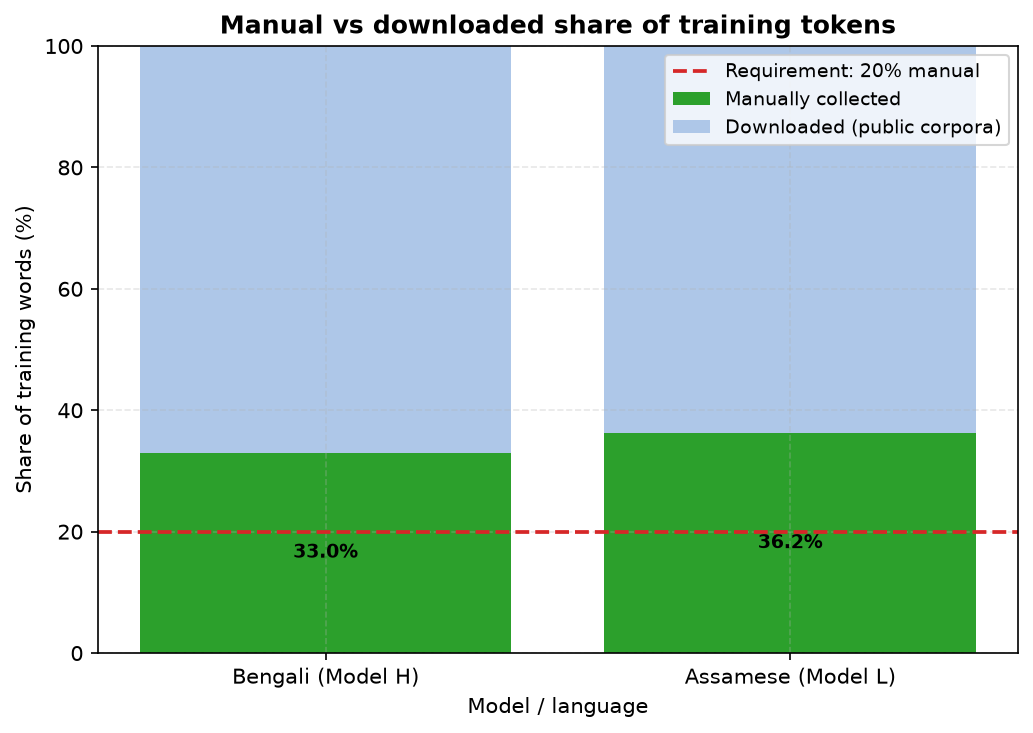
\includegraphics[width=\linewidth]{manual_fraction.png}
  \caption{Manual share of collected words}
\end{subfigure}\hfill
\begin{subfigure}[b]{0.615\linewidth}
  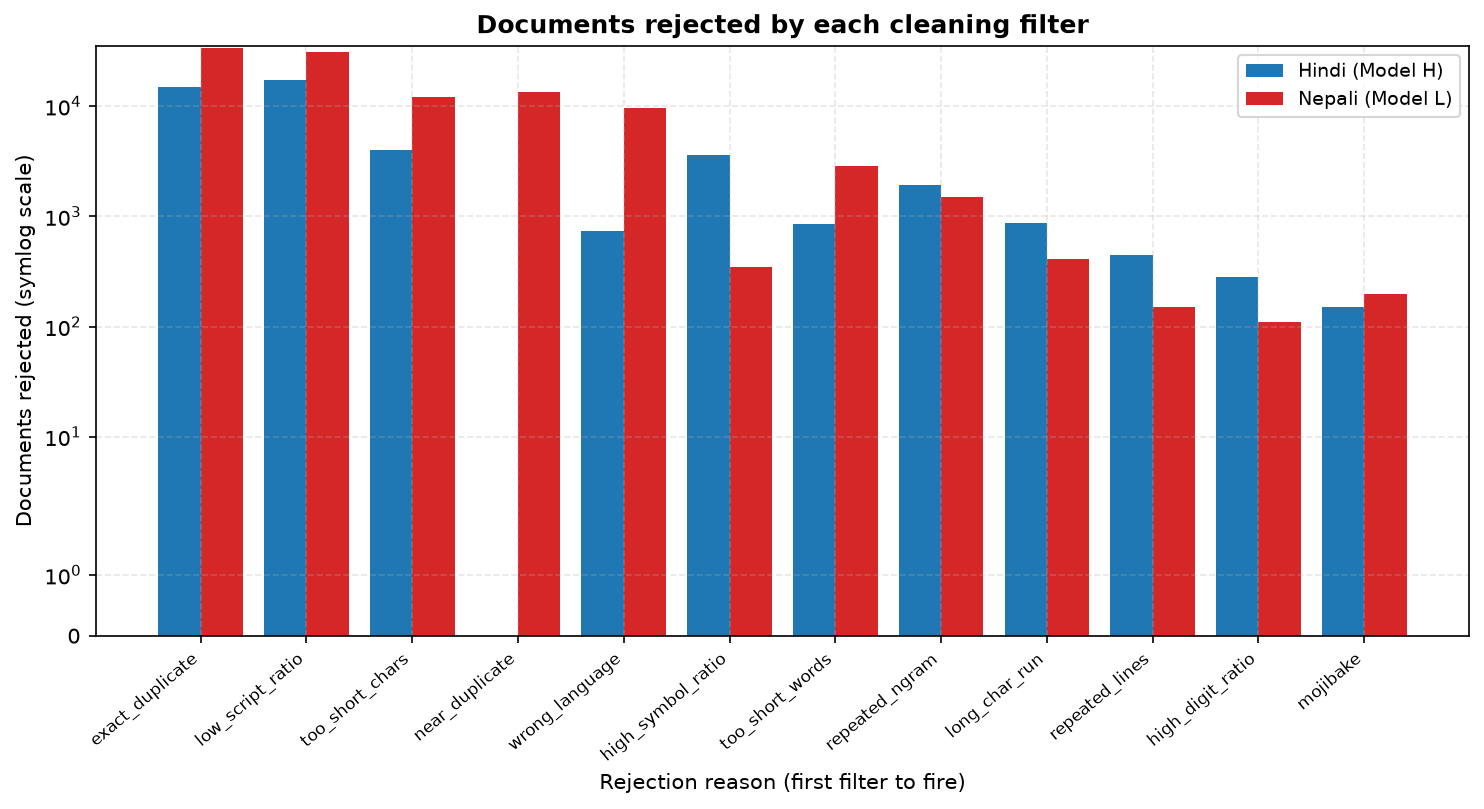
\includegraphics[width=\linewidth]{cleaning_funnel.png}
  \caption{Documents surviving each filter}
\end{subfigure}
\caption{Phase 1 corpus construction. Nepali reaches a far higher manual share, and loses more of its input to quality filtering.}
\label{fig:phase1}
\end{figure}

\subsection{Tokenizers}

Each language has its own SentencePiece Unigram tokenizer, trained only on its
own training split with \num{8000} pieces,
\texttt{character\_coverage=0.9995}, byte fallback enabled, digits split, and
\texttt{normalization\_rule\_name=identity} because the corpus is already
normalised. I chose the vocabulary size by measurement rather than assertion.
At a fixed 25M-parameter budget the embedding matrix competes directly with the
transformer layers, so candidate sizes from 5{,}000 to 10{,}000 were trained and
scored on held-out text: moving from 5{,}000 to 10{,}000 shortens sequences by
\pc{9.9} but costs 2.2M transformer parameters, roughly a tenth of the modeling
capacity. \num{8000} is the largest size at which the fertility return still
justifies the embedding spend.

\begin{table}[htbp]
\centering\small
\begin{tabular}{@{}l r r r r r@{}}
\toprule
\textbf{Vocabulary} & \num{4000} & \num{5000} & \num{6000} & \num{8000} & \num{10000} \\
\midrule
Hindi fertility  & ---   & 1.562 & 1.516 & \textbf{1.452} & 1.411 \\
Nepali fertility & 1.918 & 1.827 & 1.763 & \textbf{1.673} & 1.614 \\
Unknown rate, both & 0.000 & 0.000 & 0.000 & 0.000 & 0.000 \\
\bottomrule
\end{tabular}
\caption{Vocabulary sweep, measured on held-out documents. Bold marks the size I deployed for both models. Fertility falls monotonically with vocabulary size, and the unknown rate is zero everywhere because byte fallback makes any input representable.}
\label{tab:sweep}
\end{table}

Table~\ref{tab:sweep} records the sweep, and it contains one result I decided to
override. The selection rule --- best held-out fertility within the permitted
range --- picks \num{8000} for Hindi but \num{10000} for Nepali. I held Nepali at
\num{8000} anyway. Letting the two models differ in vocabulary size would have
confounded exactly the comparison the project exists to make, since a perplexity
gap could then be attributed to the tokenizer rather than to the data. The cost
of that decision is measurable: Nepali gives up \pc{3.7} on fertility, 1.673
against 1.614. I judged a controlled comparison worth more than that, but it is a
choice rather than a measurement, and Section~\ref{sec:tiers} depends on it.

\begin{table}[htbp]
\centering\small
\caption{Tokenizer behaviour measured on \num{3000} held-out documents per language. The two tokenizers are configured identically; the differences between them are produced by the data.}
\label{tab:tok}
\begin{tabular}{@{}l r r@{\hskip 18pt} l r r@{}}
\toprule
 & \textbf{H} & \textbf{L} & & \textbf{H} & \textbf{L} \\
\midrule
Vocabulary size          & \num{8000} & \num{8000} & Byte-fallback rate      & \pc{0.59} & \pc{0.99} \\
Fertility (tokens/word)  & 1.453      & 1.692      & Unknown rate            & 0.000     & 0.000 \\
Characters per token     & 3.537      & 3.992      & Mean piece length (ch.) & 4.666     & 5.635 \\
Bytes per token          & 8.981      & 10.657     & Script pieces           & \num{7230} & \num{7710} \\
Single-token word rate   & \pc{74.9}  & \pc{59.0}  & Latin pieces            & \num{479} & \num{4} \\
Top-1000 token coverage  & \pc{73.2}  & \pc{69.8}  & Vocabulary utilisation  & \pc{98.1} & \pc{98.2} \\
\bottomrule
\end{tabular}
\end{table}

Two rows in Table~\ref{tab:tok} matter downstream. Fertility is 1.453 for Hindi
against 1.692 for Nepali, and the single-token word rate is \pc{74.9} against
\pc{59.0}. At a fixed \num{512}-token context Model~L therefore sees fewer words
in each window, and spends more of its capacity reassembling words from pieces.
The unknown rate is exactly zero for both models, because byte fallback makes any
input representable, so the honest measure of rare material is the byte-fallback
rate: \pc{0.59} against \pc{0.99}. The Latin-piece counts, \num{479} against
\num{4}, show how much more code-mixed the Hindi sources are.

% =====================================================================
\section{Phase 2 --- Architecture, pretraining and evaluation}\label{sec:p2}
% =====================================================================

\subsection{Model and training setup}

I implemented both models from scratch in \texttt{lma/model/} as decoder-only
transformers: \num{12} layers, \num{6} heads, $d_{\text{model}}=384$,
$d_{\text{ff}}=1536$, a \num{512}-token context, dropout 0.1, learned absolute
positional embeddings and tied input and output embeddings, giving
\num{24562944} trainable parameters. I wrote the multi-head attention, the positional embeddings and the causal mask
myself, and
\texttt{scripts/test\_model.py} checks that tensor shapes are correct, that a
position's logits are unchanged by any edit to later positions, and that a
checkpoint resumes bit-identically. I trained with AdamW, batch \num{24} and
gradient accumulation \num{4}, a learning rate of $6\times10^{-4}$ decayed on a
cosine schedule to $6\times10^{-5}$ after \num{500} warmup steps, weight decay
0.1, gradient clipping 1.0, mixed precision, and \num{12000} steps. Each run
spanned two sessions because the training platform caps a session at twelve
hours; wall-clock times were \num{95004} and \num{94212} seconds, and the validation
curves are shown in Figure~\ref{fig:losscurves}.

\begin{figure}[htbp]
\centering
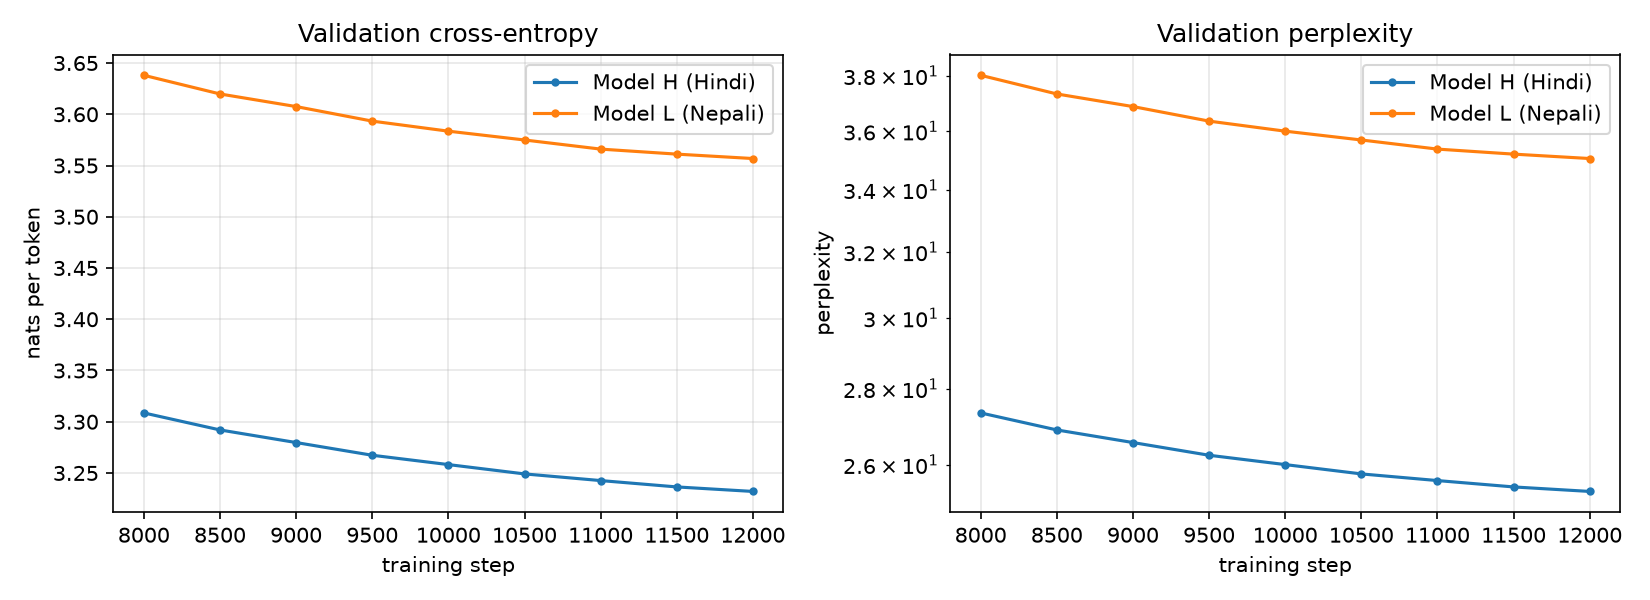
\includegraphics[width=0.96\linewidth]{phase2_loss_curves.png}
\caption{Validation loss during pretraining. The discontinuity in each curve is the twelve-hour session boundary, where training resumed from a checkpoint; resume was verified bit-exact.}
\label{fig:losscurves}
\end{figure}

\subsection{Language-modeling results}\label{sec:lm}

\begin{table}[htbp]
\centering\small
\begin{minipage}[b]{0.40\linewidth}
\centering
\begin{tabular}{@{}l r r@{}}
\toprule
 & \textbf{H} & \textbf{L} \\
\midrule
Cross-entropy (nats/tok) & 3.2152 & 3.5933 \\
Perplexity               & 24.91  & 36.35 \\
Bits-per-byte            & 0.5173 & 0.4856 \\
Bytes per token          & 8.97   & 10.68 \\
Best val.\ loss          & 3.2320 & 3.5568 \\
\bottomrule
\end{tabular}
\end{minipage}\hfill
\begin{minipage}[b]{0.575\linewidth}
\centering
\begin{tabular}{@{}l r r r r r@{}}
\toprule
\textbf{Decoding} & \textbf{chrF} & \textbf{R-L} & \textbf{BLEU} & \textbf{Rep.} & \textbf{Dist-2} \\
\midrule
\multicolumn{6}{@{}l}{\itshape Model H}\\
Greedy      & 13.57 & 10.27 & 1.07 & 0.563 & 0.288 \\
$T=0.5$     & 16.30 & 11.07 & 1.20 & 0.208 & 0.573 \\
$T=1.0$     & 18.71 &  9.82 & 0.76 & 0.002 & 0.910 \\
$T=1.5$     & 17.81 &  5.66 & 0.28 & 0.000 & 0.990 \\
\addlinespace[2pt]
\multicolumn{6}{@{}l}{\itshape Model L}\\
Greedy      & 13.91 &  3.94 & 0.00 & 0.607 & 0.323 \\
$T=0.5$     & 17.25 &  4.58 & 0.00 & 0.174 & 0.693 \\
$T=1.0$     & 19.85 &  4.57 & 0.00 & 0.000 & 0.984 \\
$T=1.5$     & 19.99 &  2.26 & 0.00 & 0.000 & 0.999 \\
\bottomrule
\end{tabular}
\end{minipage}

\caption{Left: held-out language-modeling metrics on \num{1638400} test tokens per model. Right: generation quality and diversity at four decoding settings.}
\label{tab:lm}
\end{table}

The two headline metrics rank the models differently, and the disagreement is the
most instructive result of Phase 2. Perplexity places Model~H well ahead, 24.91
against 36.35, while bits-per-byte places Model~L slightly ahead, 0.5173 against
0.4856. Both are correct. Perplexity is defined per token, and a Nepali token
carries more text than a Hindi one: 10.68 bytes against 8.97. Predicting one
Nepali token is therefore a harder prediction covering more material, and
perplexity charges Model~L for that without crediting it. Bits-per-byte
normalises by the underlying text rather than by the segmentation, which makes it
the comparable quantity across tokenizers, and by that measure the two models are
close. The generation metrics behave similarly. chrF is comparable between the
models at every temperature, but ROUGE-L is not, 10.27 against 3.94 under greedy
decoding, and BLEU-4 is 0.00 for Nepali throughout. Low absolute BLEU is expected
here, because these are open-ended continuations scored against a single
reference; the informative quantity is the gap between the models rather than the
level of either.

Greedy decoding degenerates for both models. Model~H loops on
\dev{उन्होंने 1990 में फिल्म 'दंगल' से बॉलीवुड में कदम रखा था।} and Model~L on
\dev{हातखुट्टामा हात राखेर}, with repetition rates of 0.563 and 0.607. At
$T=1.0$ repetition falls to 0.002 and 0.000 and both models produce fluent,
correctly inflected sentences whose content is invented. At 25M parameters and
590M tokens the models have acquired the syntax and register of their corpora
without acquiring reliable facts, which is also what the metric pattern in
Table~\ref{tab:lm} indicates.

\subsection{Attention analysis}

\begin{figure}[htbp]
\centering
\begin{subfigure}[b]{0.487\linewidth}
  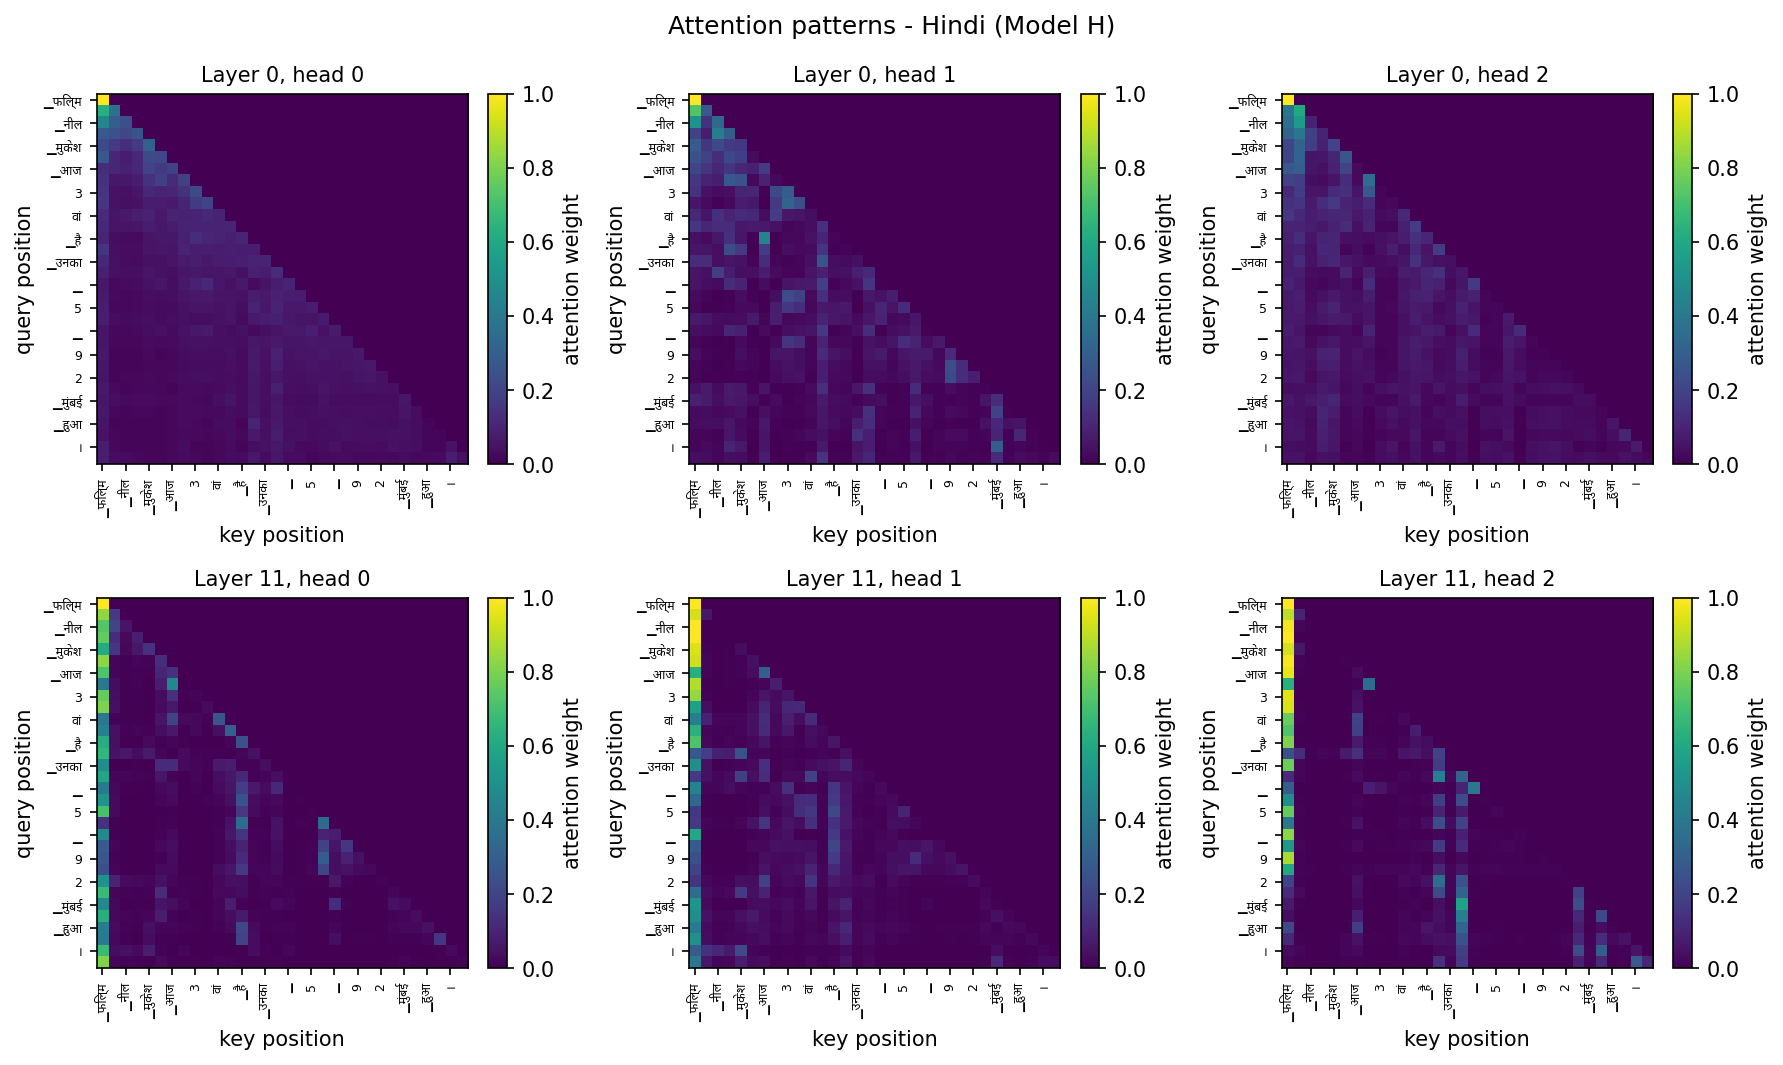
\includegraphics[width=\linewidth]{attention_heatmaps_hi.png}
  \caption{Model H}
\end{subfigure}\hfill
\begin{subfigure}[b]{0.487\linewidth}
  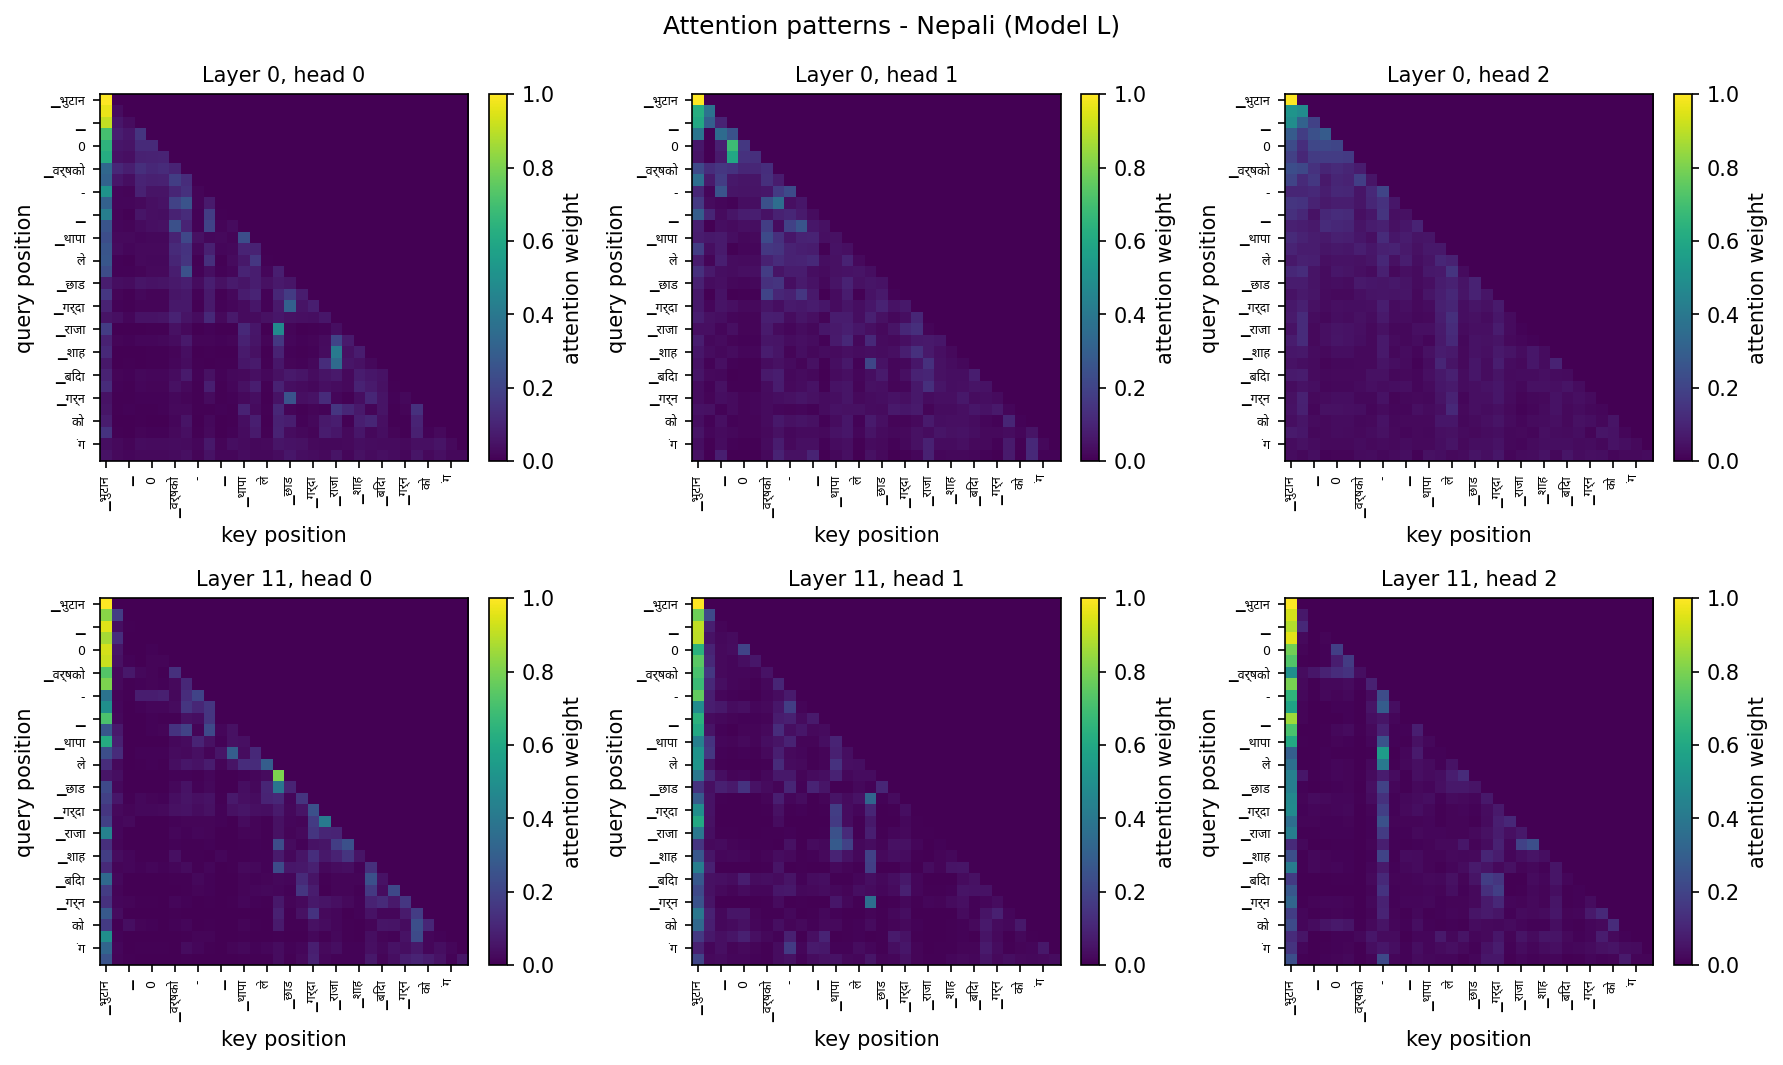
\includegraphics[width=\linewidth]{attention_heatmaps_ne.png}
  \caption{Model L}
\end{subfigure}
\caption{Pretrained attention for an early and a late layer of each model, all heads, on the same example sentence.}
\label{fig:attn2}
\end{figure}

Figure~\ref{fig:attn2} shows the heatmaps, and the per-layer statistics behind
them show both models converging on the same three-stage structure. Layers 0--2 are diffuse and long-range, with Model~H entropies of
2.999, 2.782 and 2.361 and mean attention distances of 14.95, 16.83 and 15.78
positions. The middle layers contract sharply: Model~H falls to distances of
7.51, 7.54, 7.37 and 6.86 across layers 3--6 and reaches its lowest entropy,
1.241, at layer 7. Layers 9--11 spread out again, up to a distance of 21.27.
Nepali follows the same shape with a tighter middle, reaching 4.48 at layer 5.
Classifying all \num{72} heads gives \num{10} local, \num{48} long-range and
\num{14} diffuse for Model~H, against \num{15}, \num{42} and \num{15} for
Model~L, so the two models divide labour across depth in much the same way
despite never sharing data.

% =====================================================================
\section{Phase 3 --- Reasoning finetuning and attention}\label{sec:p3}
% =====================================================================

\subsection{The synthetic reasoning dataset}

Each model is finetuned on its own synthetic dataset, which I generate
programmatically with \texttt{scripts/generate\_reasoning\_data.py} so that ground
truth is known by construction. Each of the \num{20000} examples per language states a chain of
comparisons and asks which entity lies at one end of it, for example
\dev{मोहन श्याम से अमीर है। महेश मोहन से अमीर है। सबसे अमीर कौन है? उत्तर -} with
answer \dev{महेश}. Variety comes from four comparison dimensions --- age, height,
speed and wealth --- chain lengths of two to four entities, and two question
polarities. I control leakage by reserving \pc{20} of entity names for evaluation only, and the checks in Table~\ref{tab:rdata} report no duplicate
prompts, no train--eval prompt overlap and no chain signature shared between the
splits. Every answer is a single token under both tokenizers, which makes exact
match an unambiguous measure.

\begin{table}[htbp]
\centering\small
\caption{Composition of the two synthetic reasoning datasets, and the leakage checks run against them.}
\label{tab:rdata}
\begin{tabular}{@{}l r r@{\hskip 18pt} l r r@{}}
\toprule
 & \textbf{H} & \textbf{L} & & \textbf{H} & \textbf{L} \\
\midrule
Total examples        & \num{20000} & \num{20000} & Unique prompts            & \num{20000} & \num{20000} \\
Train / val / test    & 16k/2k/2k   & 16k/2k/2k   & Duplicate prompts         & 0 & 0 \\
Chain length 2 / 3 / 4 & \num{5470}/\num{7480}/\num{7050} & \num{4349}/\num{8010}/\num{7641} & Train--eval prompt overlap & 0 & 0 \\
Dimensions            & 4 & 4 & Chain-signature overlap   & 0 & 0 \\
Shared entities       & \num{34} & \num{26} & Train chain signatures    & \num{12426} & \num{11264} \\
Held-out distractors  & \num{8}  & \num{7}  & Eval chain signatures     & \num{3337} & \num{3139} \\
Mean sequence tokens  & 22.45 & 24.01 & Single-token answers       & \pc{100} & \pc{100} \\
\bottomrule
\end{tabular}
\end{table}

\subsection{Finetuning}

I finetune each model from its own Phase 2 checkpoint at step \num{12000}, with
its own tokenizer and vocabulary frozen and no exposure to the other language.
Loss is computed on the answer span only. The settings are batch \num{32}, a
learning rate of $5\times10^{-5}$ decayed on a cosine schedule to
$5\times10^{-6}$ after \num{100} warmup steps, weight decay 0.1,
$\beta=(0.9,0.95)$, gradient clipping 1.0, a maximum sequence length of \num{64},
mixed precision, and three epochs, which is \num{1500} steps. The best
answer-span validation loss was 0.00458 for Model~H and 0.00243 for Model~L,
reached in 113 and 124 seconds, roughly \num{840} times less wall-clock compute
than pretraining. Figure~\ref{fig:ft} shows both curves.

\begin{figure}[htbp]
\centering
\begin{subfigure}[b]{0.435\linewidth}
  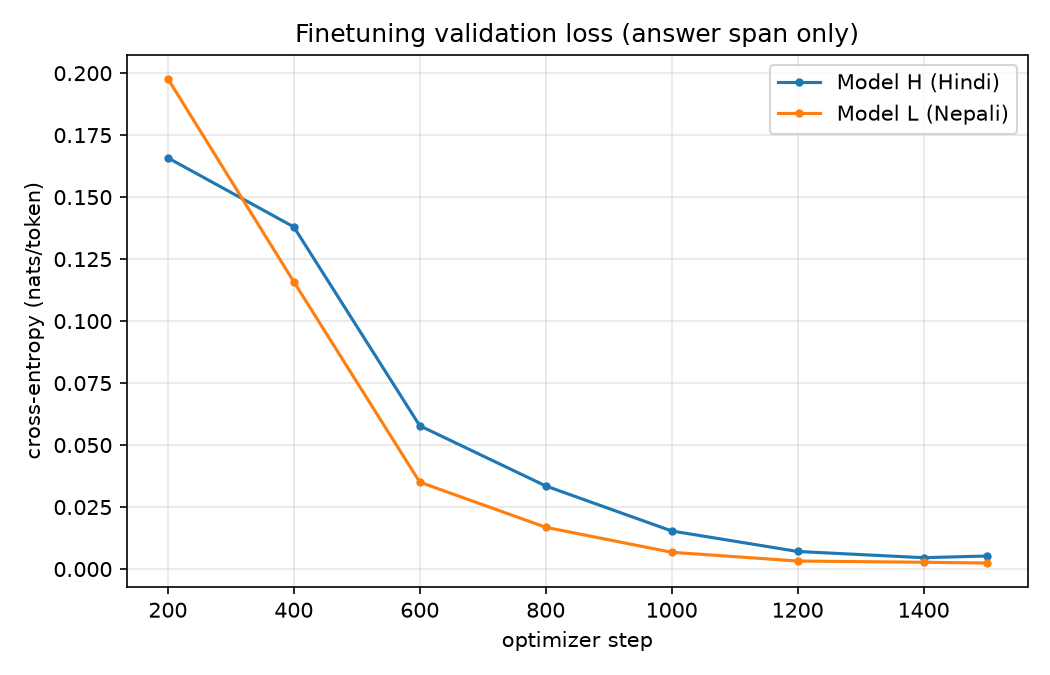
\includegraphics[width=\linewidth]{phase3_finetune_curves.png}
  \caption{Finetuning validation loss}
\end{subfigure}\hfill
\begin{subfigure}[b]{0.535\linewidth}
  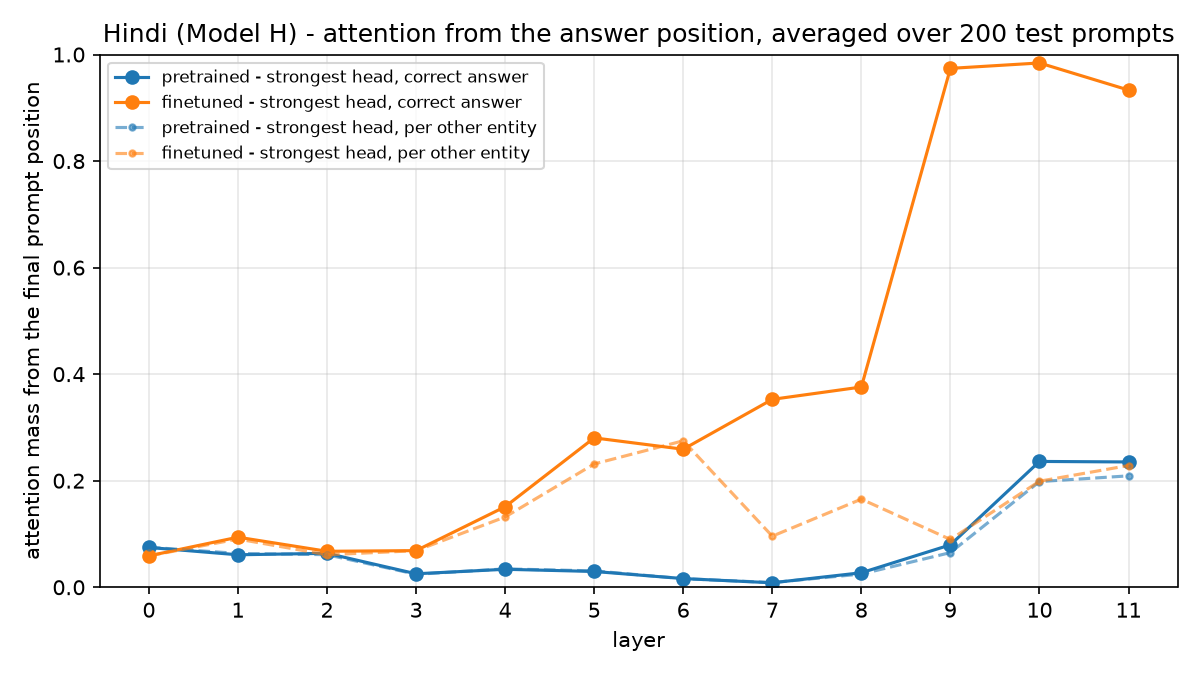
\includegraphics[width=\linewidth]{reasoning_answer_attention_hi.png}
  \caption{Attention on the answer entity, Model H}
\end{subfigure}
\caption{Left: answer-span validation loss during finetuning. Right: the share of a head's attention mass falling on the correct answer entity, before and after finetuning.}
\label{fig:ft}
\end{figure}

\subsection{Reasoning results}

\begin{table}[htbp]
\centering\small
\caption{Pretrained against finetuned performance on the held-out synthetic test set, \num{2000} examples per language, with the distribution of error types.}
\label{tab:reason}
\begin{tabular}{@{}l r r@{\hskip 10pt} r r@{}}
\toprule
 & \multicolumn{2}{c}{\textbf{Model H}} & \multicolumn{2}{c}{\textbf{Model L}} \\
\cmidrule(r){2-3}\cmidrule(l){4-5}
 & pretrained & finetuned & pretrained & finetuned \\
\midrule
Exact match                     & 0.0460 & \textbf{0.9965} & 0.0025 & \textbf{0.9985} \\
Constrained accuracy            & 0.2600 & 0.9965 & 0.2180 & 0.9985 \\
Answer mean log-prob            & $-5.608$ & $-0.015$ & $-6.203$ & $-0.009$ \\
Answer perplexity               & 272.57 & 1.0155 & 494.12 & 1.0095 \\
\addlinespace[2pt]
Chain length 2 (1 hop)          & 0.0311 & 1.0000 & 0.0000 & 1.0000 \\
Chain length 3 (2 hops)         & 0.0681 & 1.0000 & 0.0026 & 0.9987 \\
Chain length 4 (3 hops)         & 0.0354 & 0.9905 & 0.0038 & 0.9975 \\
Chance baseline (overall)       & \multicolumn{2}{c}{0.3483} & \multicolumn{2}{c}{0.3381} \\
\addlinespace[2pt]
Errors examined                 & \num{1908} & \num{7} & \num{1995} & \num{3} \\
\quad off-chain entity          & \pc{78.1} & \pc{0} & \pc{96.1} & \pc{0} \\
\quad wrong entity on chain     & \pc{16.6} & \pc{100} & \pc{3.7} & \pc{100} \\
\quad inverted comparison       & \pc{5.3}  & \pc{0} & \pc{0.2} & \pc{0} \\
\bottomrule
\end{tabular}
\end{table}

Table~\ref{tab:reason} gives the results. Both models move from near-zero to
near-ceiling exact match, and both clear the per-chain-length chance baselines by margins between 0.50 and 0.75. The leakage
checks and the evaluation-only entity pool rule out memorisation of test items.
The error taxonomy is more revealing than the accuracy figures. Before
finetuning, \pc{78.1} of Model~H's errors and \pc{96.1} of Model~L's name an
entity that does not appear in the chain at all, which indicates that the models
were not attempting the task rather than attempting and failing it; the small
inverted-comparison fractions, \pc{5.3} against \pc{0.2}, suggest Model~H
occasionally grasped the relation and reversed its direction where Model~L
essentially never did. Constrained accuracy separates the two failure modes:
restricting the prediction to entities named in the prompt lifts the pretrained
models from 0.046 and 0.0025 to 0.260 and 0.218, so a substantial part of the
pretrained failure was formatting rather than reasoning. After finetuning, every
remaining error --- seven for Model~H and three for Model~L --- names an entity
that is on the chain but in the wrong position, and all of them occur at chain
length four.

A representative Model~H failure is
\dev{अनिल अशोक से लंबा है। दीपक अनिल से लंबा है। अशोक सूरज से लंबा है। सबसे छोटा कौन है?},
answered \dev{अशोक} where the correct answer is \dev{सूरज}: the model stopped one
hop short of the end of the chain. All three Model~L failures involve the pair
\dev{विकास} and \dev{बिकास}, which are spelling variants of the same name that the
generator treated as distinct entities. That is a dataset artefact rather than a
reasoning failure, and it accounts for the whole of Model~L's residual error.

\subsection{Attention before and after finetuning}

\begin{figure}[htbp]
\centering
\begin{subfigure}[b]{0.487\linewidth}
  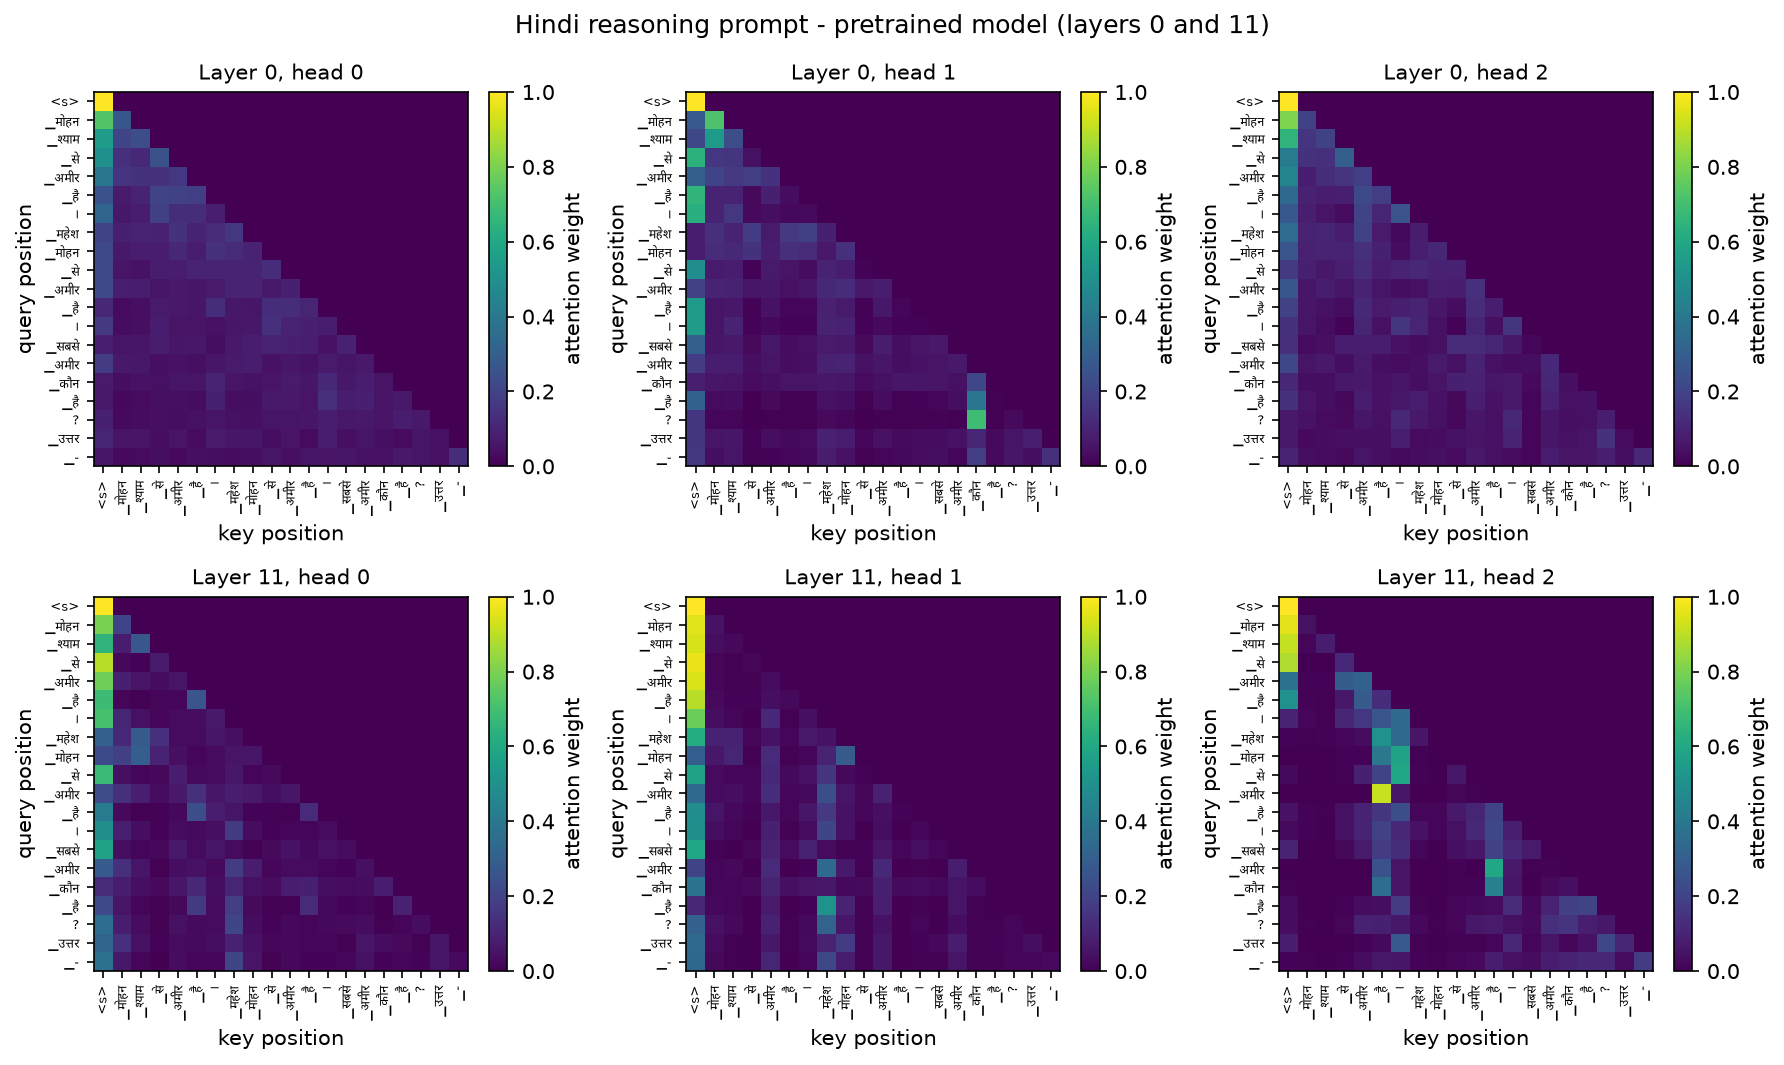
\includegraphics[width=\linewidth]{reasoning_attention_pretrained_hi.png}
  \caption{Model H, pretrained}
\end{subfigure}\hfill
\begin{subfigure}[b]{0.487\linewidth}
  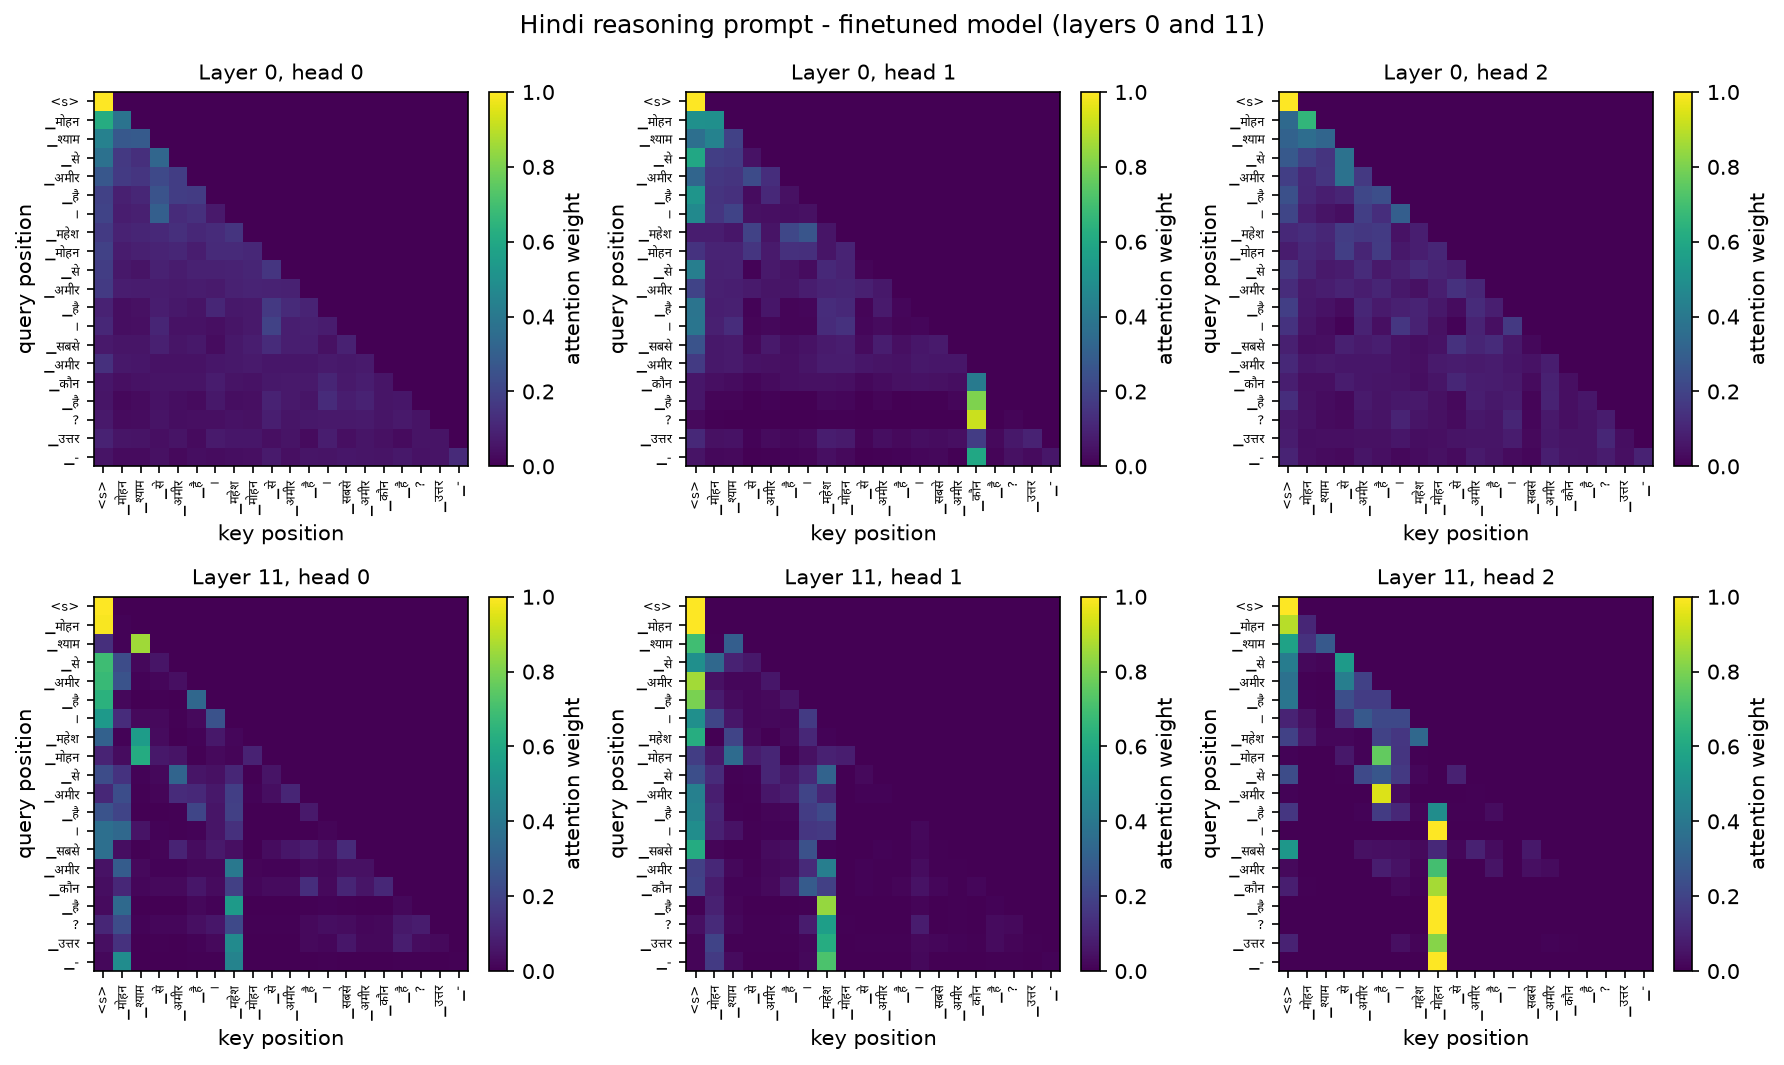
\includegraphics[width=\linewidth]{reasoning_attention_finetuned_hi.png}
  \caption{Model H, finetuned}
\end{subfigure}\\[4pt]
\begin{subfigure}[b]{0.487\linewidth}
  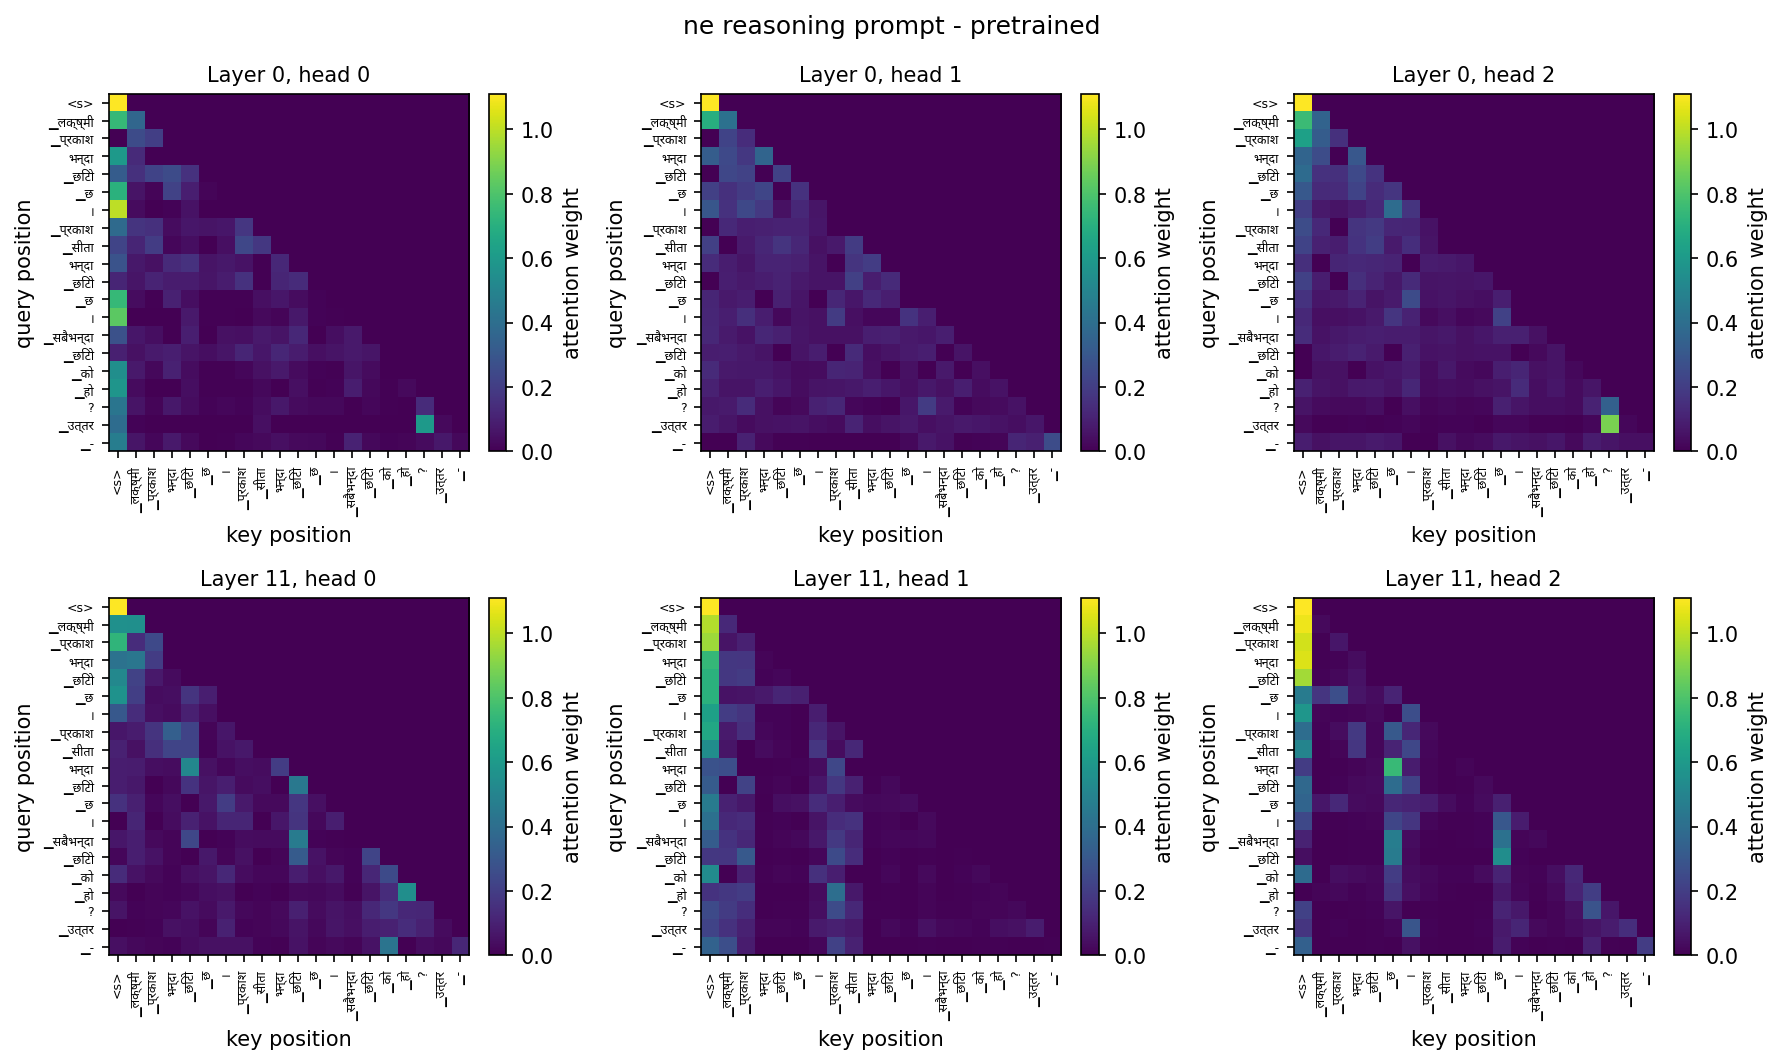
\includegraphics[width=\linewidth]{reasoning_attention_pretrained_ne.png}
  \caption{Model L, pretrained}
\end{subfigure}\hfill
\begin{subfigure}[b]{0.487\linewidth}
  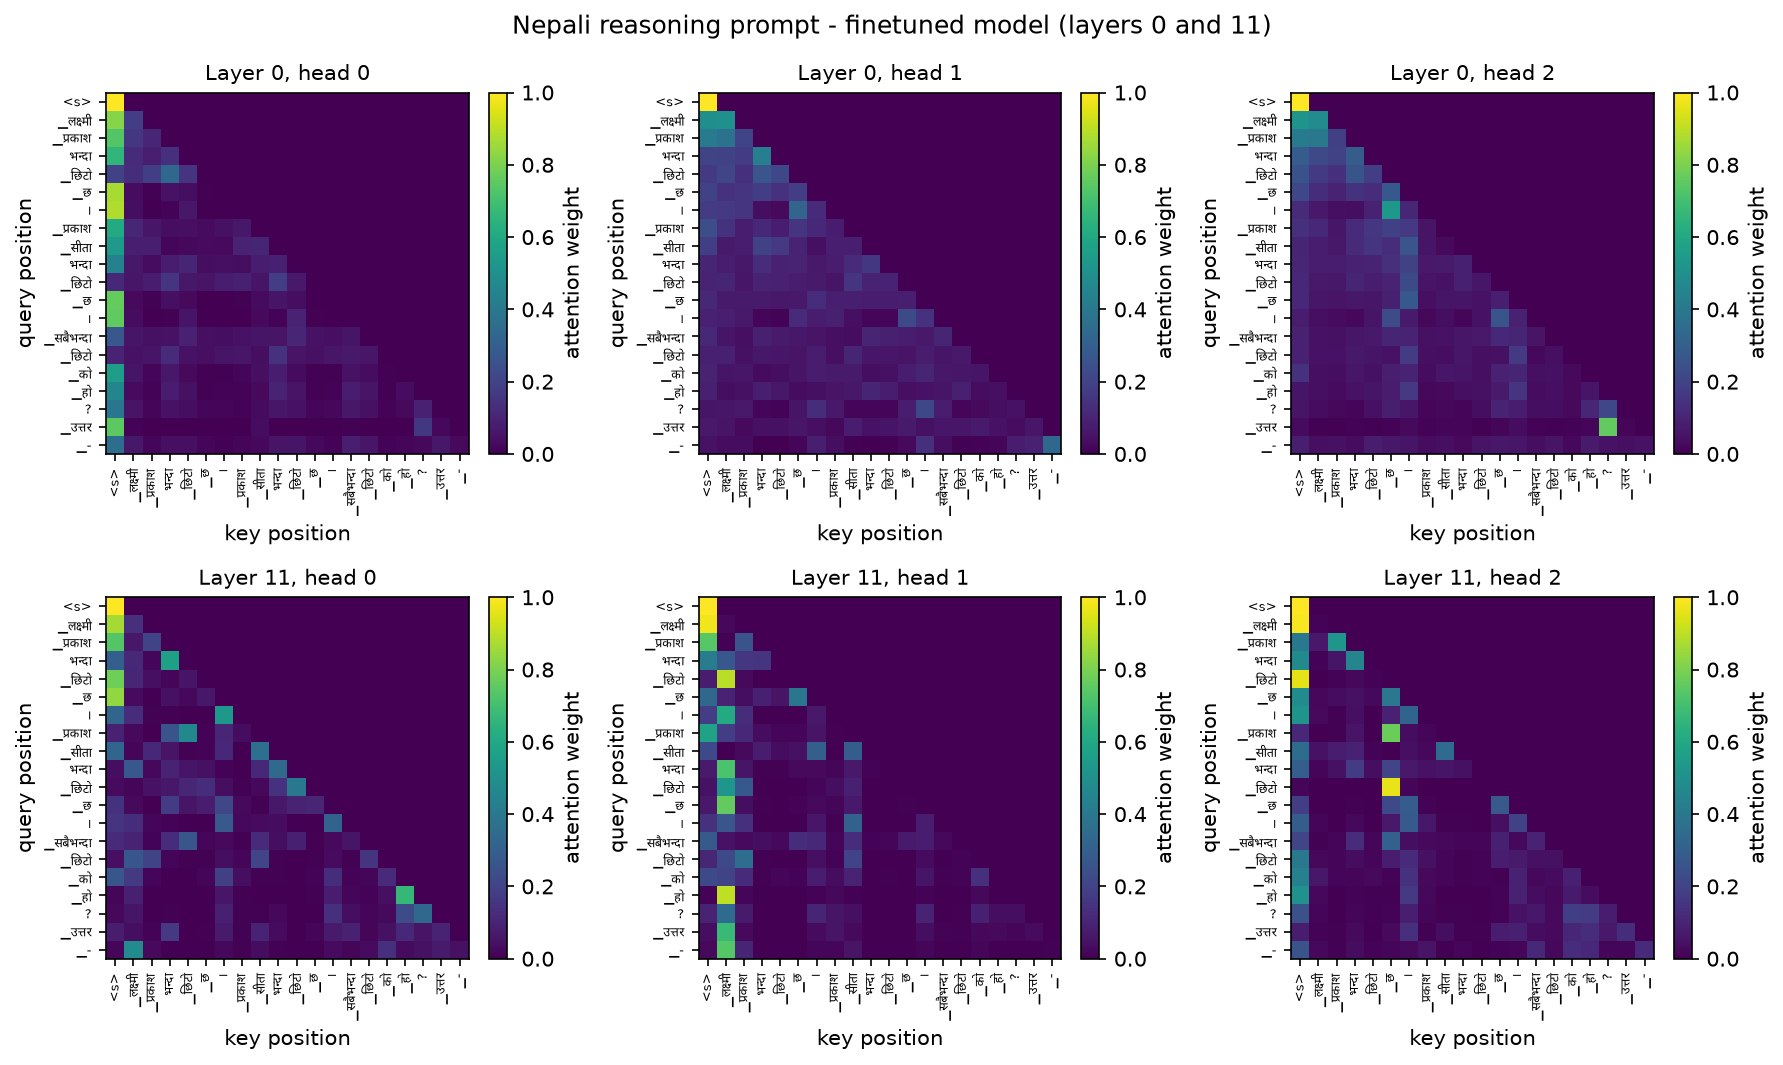
\includegraphics[width=\linewidth]{reasoning_attention_finetuned_ne.png}
  \caption{Model L, finetuned}
\end{subfigure}
\caption{Attention on a comparative-reasoning prompt for an early and a late layer of each model, before and after finetuning.}
\label{fig:attn3}
\end{figure}

\begin{table}[htbp]
\centering\small
\caption{Attention statistics averaged over \num{200} reasoning prompts per model, before and after finetuning.}
\label{tab:attn3}
\begin{tabular}{@{}l r r@{\hskip 10pt} r r@{}}
\toprule
 & \multicolumn{2}{c}{\textbf{Model H}} & \multicolumn{2}{c}{\textbf{Model L}} \\
\cmidrule(r){2-3}\cmidrule(l){4-5}
 & pretrained & finetuned & pretrained & finetuned \\
\midrule
Local heads (of \num{72})       & 34 & 45 & 29 & 36 \\
Long-range heads                & 32 & 23 & 36 & 29 \\
Diffuse heads                   &  6 &  4 &  7 &  7 \\
\addlinespace[2pt]
Layer 0 mean distance           & 5.35 & 5.04 & 5.59 & 5.56 \\
Layer 8 mean distance           & 4.85 & 3.64 & 6.15 & 4.61 \\
Layer 11 mean distance          & 5.70 & 5.87 & 6.23 & 6.32 \\
Layer 0 mean entropy            & 1.878 & 1.895 & 1.949 & 1.950 \\
Layer 11 mean entropy           & 1.441 & 1.159 & 1.642 & 1.451 \\
\addlinespace[2pt]
Max head attention on answer, layer 9  & 0.080 & \textbf{0.974} & 0.228 & \textbf{0.956} \\
\quad same head, on a distractor entity & 0.065 & 0.090 & 0.179 & 0.116 \\
Max head attention on answer, layer 10 & 0.236 & \textbf{0.984} & 0.217 & \textbf{0.980} \\
\quad same head, on a distractor entity & 0.198 & 0.199 & 0.179 & 0.424 \\
\bottomrule
\end{tabular}
\end{table}

Figure~\ref{fig:attn3} and Table~\ref{tab:attn3} compare attention before and
after finetuning, and show three measurable changes. First, heads become more
local: Model~H shifts from \num{34} to \num{45} local heads and from \num{32} to
\num{23} long-range ones, and Model~L from \num{29} to \num{36} and from \num{36}
to \num{29}. Mean attention distance falls in eleven of twelve layers for
Model~H and ten of twelve for Model~L, with the largest reductions in the
middle-to-late layers ($-1.22$ positions at layer 8 for Model~H, $-1.54$ for
Model~L). Second, late-layer attention sharpens: entropy at layer 11 falls from
1.441 to 1.159 and from 1.642 to 1.451, while layer 0 barely moves. Third, and
most strikingly, individual heads in layers 9--11 become answer detectors. The
most answer-focused head at layer 10 moves from 0.236 to 0.984 of its attention
mass on the correct entity for Model~H, and from 0.217 to 0.980 for Model~L.
This is selectivity rather than a general increase in attention to entities: at
layer 9, Model~H's most answer-focused head moves from 0.080 on the answer and
0.065 on a distractor to 0.974 and 0.090.

% =====================================================================
\section{The two resource tiers compared}\label{sec:tiers}
% =====================================================================

\subsection{Data scale and quality}

Scale is nearly equal and, on raw count, favours Nepali: \num{612476098} training
tokens against \num{580162728}. Quality does not. Hindi retained \pc{93.7} of its
input documents against Nepali's \pc{88.0}, and Table~\ref{tab:sources} shows
where the difference lies: Nepali lost \num{9723} documents to wrong-language
detection against \num{758}, \num{31028} to low script ratio against
\num{17453}, and a further \num{13495} to near-duplicate detection that Hindi did
not require. Source diversity also differs. Model~H draws on seven sources
including a large curated public corpus, while Model~L draws on three, of which a
single bulk manual source supplies \pc{52} of its words. The corpora differ in
character inventory as well, \num{6395} distinct characters against \num{3093},
and in Latin content, \pc{2.09} against \pc{0.48}, reflecting how much more
code-mixed the Hindi web and news material is.

\subsection{Language modeling against reasoning}

Language modeling separates the tiers, but only on tokenizer-dependent
metrics. Perplexity differs substantially, 24.91 against 36.35, and greedy
ROUGE-L by more than a factor of two, 10.27 against 3.94, yet bits-per-byte and
chrF are close, with bits-per-byte marginally favouring Model~L. Reasoning does
not separate the tiers at all once finetuned: 0.9965 against 0.9985, with
Model~L nominally ahead. The asymmetry follows from what each task demands.
Open-ended next-token prediction over natural text rewards corpus breadth and
cleanliness, which is exactly where the two corpora differ. A templated
comparison task over four dimensions with single-token answers is narrow enough
that 590M pretraining tokens of either quality provide a sufficient foundation,
so the task saturates and its ceiling conceals any residual tier difference.

\subsection{Dominant factors for the lower-resource model}

Tokenizer fertility is the dominant factor. With vocabulary size,
architecture, context length and training recipe all held equal, Nepali's
fertility of 1.692 against Hindi's 1.453 means Model~L's \num{512}-token window
covers about \pc{14} less text, and its single-token word rate of \pc{59.0}
against \pc{74.9} means it must assemble a far larger share of words from
multiple pieces. Byte fallback is secondary, \pc{0.99} against \pc{0.59},
indicating that more rare and out-of-distribution material reaches the model as
raw bytes. Both are consequences of the corpus rather than of the tokenizer
configuration, which was identical. Fertility is also what produces the
perplexity and bits-per-byte disagreement of Section~\ref{sec:lm}: the per-token
metric measures segmentation as much as modeling ability, and once segmentation
is normalised away the apparent gap largely disappears.

\subsection{Why the differences arise}

The design supports the attribution. The two models share an identical \num{24562944}-parameter
architecture, an identical tokenizer algorithm and vocabulary size, identical
optimizer settings, step count and token budget, the same seed and the same
evaluation code, and the independence checks confirm that no document, tokenizer
artifact or weight is shared. Every difference reported here therefore originates
in the corpora. The chain of evidence runs from the cleaning-funnel asymmetry,
through the resulting fertility gap, to the perplexity difference, with
bits-per-byte acting as the control that shows how much of that difference is
segmentation rather than modeling. The attention statistics support the Phase 3
conclusion independently of accuracy, since answer-selective heads emerge in
layers 9--11 of both models. The weaker claims are those resting on single runs:
the direction of the bits-per-byte result and the small differences between the
models' head classifications should be read as observations, not as established
effects.

\subsection{Limitations}

Each configuration was trained once, so no variance estimate is available and
differences of the size that run-to-run noise produces should not be read as
effects. At 25M parameters and 590M tokens the absolute generation quality of
both models is low, which makes BLEU-4 uninformative and limits what the
qualitative samples can show. The reasoning task is templated and narrow, and its
saturation means it cannot measure a resource gap. Classifying sources as manual
or downloaded involves judgement. The attention results are correlational: they
show where attention mass moves, not that the model's answer depends on those
heads, which would require ablating them.

% =====================================================================
\section{Bonus ablation --- no positional embeddings (Model H)}
% =====================================================================

\begin{table}[htbp]
\centering\small
\caption{Model H retrained with the positional-embedding table removed, compared against the standard model on the same data, steps, prompts and decoding settings.}
\label{tab:abl}
\begin{tabular}{@{}l r r@{\hskip 18pt} l r r@{}}
\toprule
 & \textbf{Standard} & \textbf{No pos.} & & \textbf{Standard} & \textbf{No pos.} \\
\midrule
Trainable parameters   & \num{24562944} & \num{24366336} & Val.\ loss @ step \num{3000} & 3.6004 & 3.6493 \\
Optimizer steps        & \num{12000} & \num{12000}       & Val.\ loss @ step \num{12000}& 3.2320 & 3.2703 \\
Cross-entropy          & 3.2152 & 3.2515                 & Greedy repetition rate       & 0.563  & 0.615 \\
Perplexity             & 24.91  & 25.83                  & Greedy chrF / ROUGE-L        & 13.57 / 10.27 & 12.44 / 9.08 \\
Bits-per-byte          & 0.5173 & 0.5231                 & Local / long-range heads     & 10 / 48 & 12 / 37 \\
Layer 0 distance / entropy & 14.95 / 2.999 & 14.27 / 2.809 & Diffuse heads              & 14 & 23 \\
\bottomrule
\end{tabular}
\end{table}

\begin{figure}[htbp]
\centering
\begin{subfigure}[b]{0.435\linewidth}
  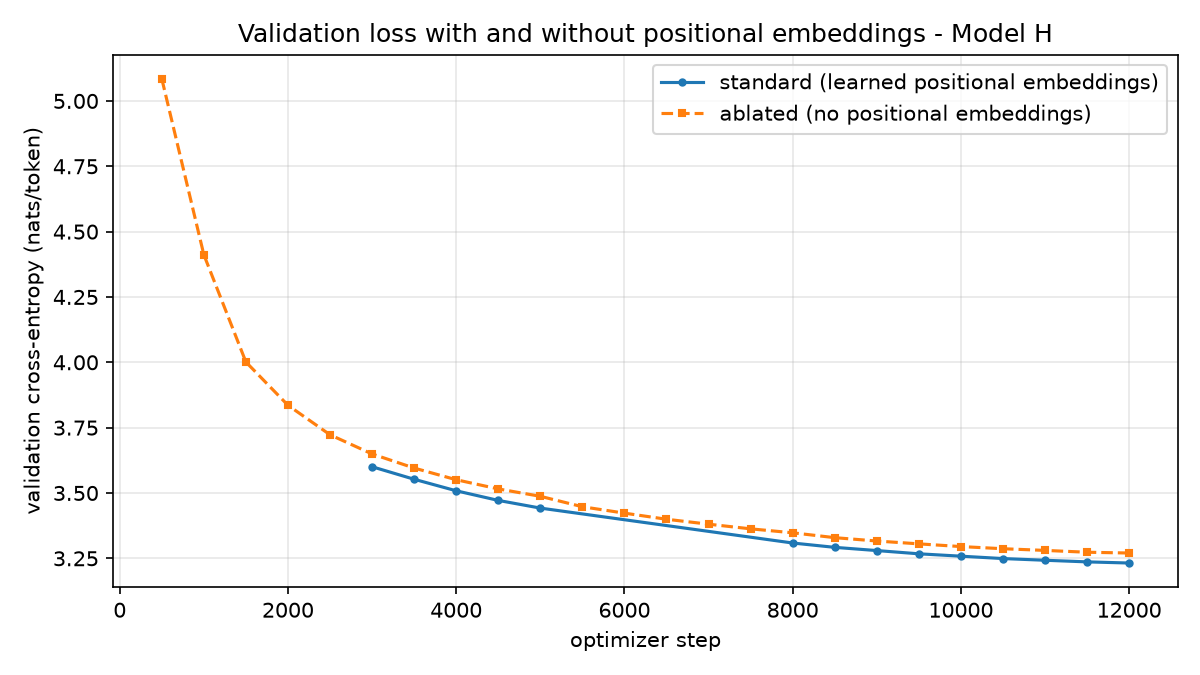
\includegraphics[width=\linewidth]{bonus_ablation_loss_hi.png}
  \caption{Validation loss}
\end{subfigure}\hfill
\begin{subfigure}[b]{0.535\linewidth}
  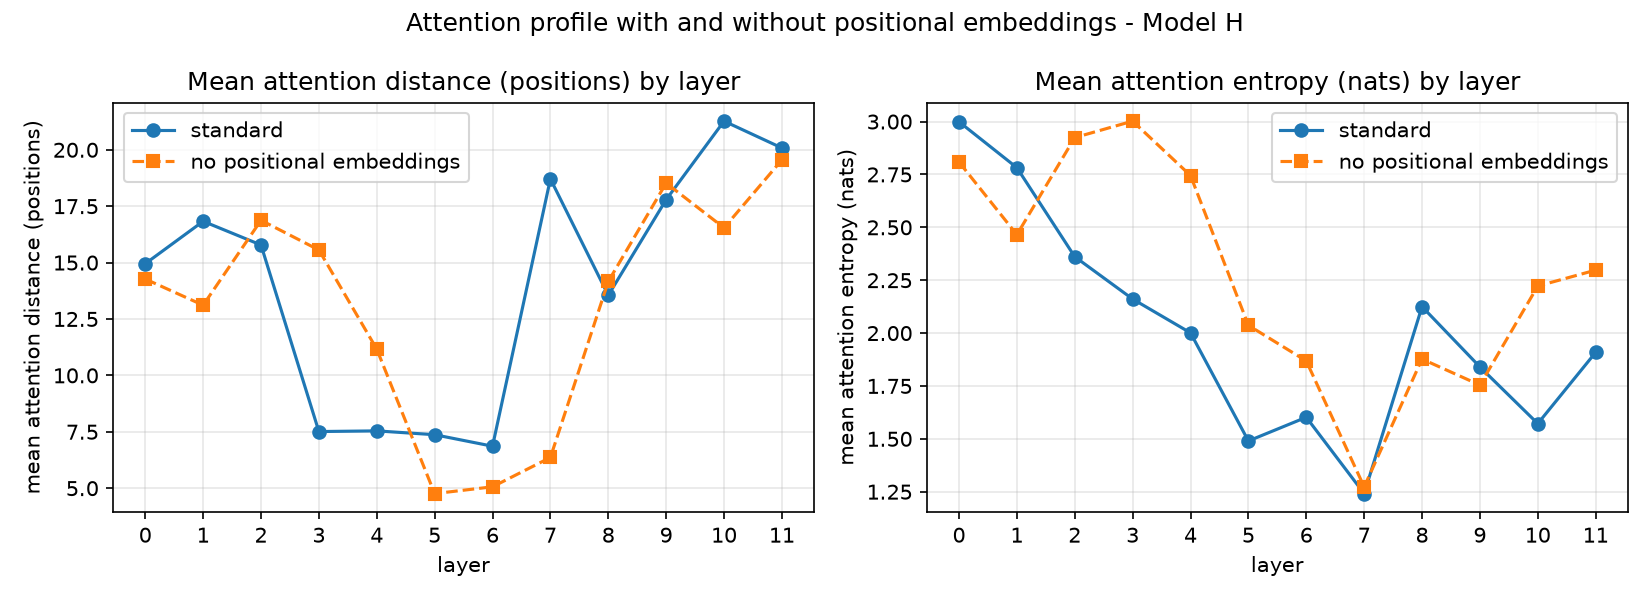
\includegraphics[width=\linewidth]{bonus_ablation_attention_hi.png}
  \caption{Attention profile}
\end{subfigure}
\caption{Effect of removing positional embeddings from Model H. The validation-loss gap narrows as training proceeds.}
\label{fig:abl}
\end{figure}

As an optional bonus, I retrained Model~H with
\texttt{use\_positional\_embeddings=False} and put through the full Phase 2
evaluation suite on the same data, steps, prompts, decoding settings and
attention sample; Table~\ref{tab:abl} and Figure~\ref{fig:abl} report the
comparison. The cost is small: perplexity rises from 24.91 to 25.83, a
factor of 1.04, and bits-per-byte from 0.5173 to 0.5231. The reason the cost is
not larger is that removing the table does not make the stack order-blind. A
single attention layer with no positional signal does see the preceding tokens as
an unordered set, but under the causal mask each position's hidden state
summarises a prefix of a different length, so a second layer can recover order
from prefix length; \texttt{scripts/test\_reasoning.py} verifies both halves of
this on small models. The narrowing loss gap is consistent with it, falling from
$+0.0489$ nats at step \num{3000} to $+0.0383$ at step \num{12000}. Layer 0 is
the only layer with no earlier layer to reconstruct from, and it is where the
loss shows: entropy falls from 2.999 to 2.809, while across all heads the diffuse
count rises from \num{14} to \num{23} and the long-range count falls from
\num{48} to \num{37}. Behaviourally, greedy repetition rises from 0.563 to 0.615
and greedy ROUGE-L falls from 10.27 to 9.08.

% =====================================================================
\section{Reproducibility and artifacts}\label{sec:repro}
% =====================================================================

The README gives full reproduction steps. The pipeline runs as component
self-tests, corpus build, tokenizer training with the vocabulary sweep, exact
token counting, the independence check, pretraining, evaluation, reasoning-data
generation, finetuning and Phase 3 evaluation. Every stage is seeded with
\num{20260812}, and checkpoints are resume-capable with resume verified
bit-exact. \texttt{scripts/check\_phase1.py}, \texttt{check\_phase2.py} and
\texttt{check\_phase3.py} verify the deliverables of each phase and exit non-zero
on a missing artifact. Table~\ref{tab:drive} lists the large artifacts held on
Google Drive, all with public viewing enabled.

\begin{table}[htbp]
\centering\small
\caption{Large artifacts, held on Google Drive with public viewing rather than committed to git.}
\label{tab:drive}
\begin{tabular}{@{}l l r l@{}}
\toprule
\textbf{Artifact} & \textbf{Phase} & \textbf{Size} & \textbf{Link} \\
\midrule
Hindi processed splits (H)         & 1 & 5.23\,GB & \href{https://drive.google.com/drive/folders/1ggiw-RzYTUgkXLhky2u73tObkw7MKbJT?usp=drive_link}{\texttt{Phase1-Processed/hindi/}} \\
Nepali processed splits (L)        & 1 & 6.61\,GB & \href{https://drive.google.com/drive/folders/1ggiw-RzYTUgkXLhky2u73tObkw7MKbJT?usp=drive_link}{\texttt{Phase1-Processed/nepali/}} \\
Hindi manual sources               & 1 & 1.31\,GB & \href{https://drive.google.com/drive/folders/1ggiw-RzYTUgkXLhky2u73tObkw7MKbJT?usp=drive_link}{\texttt{Phase1-Manual/hindi/}} \\
Nepali manual sources              & 1 & 4.36\,GB & \href{https://drive.google.com/drive/folders/1ggiw-RzYTUgkXLhky2u73tObkw7MKbJT?usp=drive_link}{\texttt{Phase1-Manual/nepali/}} \\
Public source corpora              & 1 & 11.56\,GB & \href{https://drive.google.com/drive/folders/1ggiw-RzYTUgkXLhky2u73tObkw7MKbJT?usp=drive_link}{\texttt{Phase1-Sources/}} \\
Pretrained checkpoints (H and L)   & 2 & 590\,MB  & \href{https://drive.google.com/drive/folders/1YymXv5SGVEQbEtiJTiNZs8Wae7JfpZmk?usp=drive_link}{\texttt{Phase2-Checkpoints/}} \\
Finetuned checkpoints (H and L)    & 3 & 590\,MB  & \href{https://drive.google.com/drive/folders/1DWhTSk7cBxHHVn0_c7qcagOVYeVsIwWI?usp=drive_link}{\texttt{Phase3-Finetuned/}} \\
\bottomrule
\end{tabular}
\end{table}

% =====================================================================
\section*{Reflection}
% =====================================================================

Three things in this project turned out differently from what I expected. The
first was the twelve-hour session cap on the training platform, which meant
neither pretraining run could finish in one sitting. What began as an
inconvenience forced the checkpointing to be genuinely correct rather than
approximately correct, including a test that a resumed run reproduces the
original bit for bit, and that test caught problems a loss curve would have
hidden.

The second was the disagreement between perplexity and bits-per-byte. I had
assumed that a model trained on a cleaner and more varied corpus would win on any
reasonable measure, and instead the two metrics ranked the models in opposite
directions. Working out why --- that perplexity is denominated in tokens, and the
two tokenizers do not produce comparable tokens --- changed how I read every
subsequent number, and it is the single result I would keep if I could keep only
one.

The third was the positional-embedding ablation, which cost far less than I
expected. Reasoning about why a causally masked stack can reconstruct order from
prefix length, and then confirming it on small models, taught me more about what
positional embeddings actually contribute than the standard model did.

With more compute I would train each configuration several times to separate real
effects from run-to-run variation, and replace the synthetic reasoning task with
one that does not saturate.

\end{document}
